%!TEX root = ../thesis.tex
% ******************************* Thesis Appendix A ****************************
\chapter{Extended Data}

\section{LTLM J-V, Samples C and D}
For J-V plots, $1$ \si{\pico\ampere} error bars are included, resulting in notable regions of error at low voltage and low temperature.
\label{app:LTLM_J_V_data}
\subsection{Sample C: 10 \si{\volt} range}
\label{app:J_V_sample_C}
\begin{figure}[h]
    \centering
    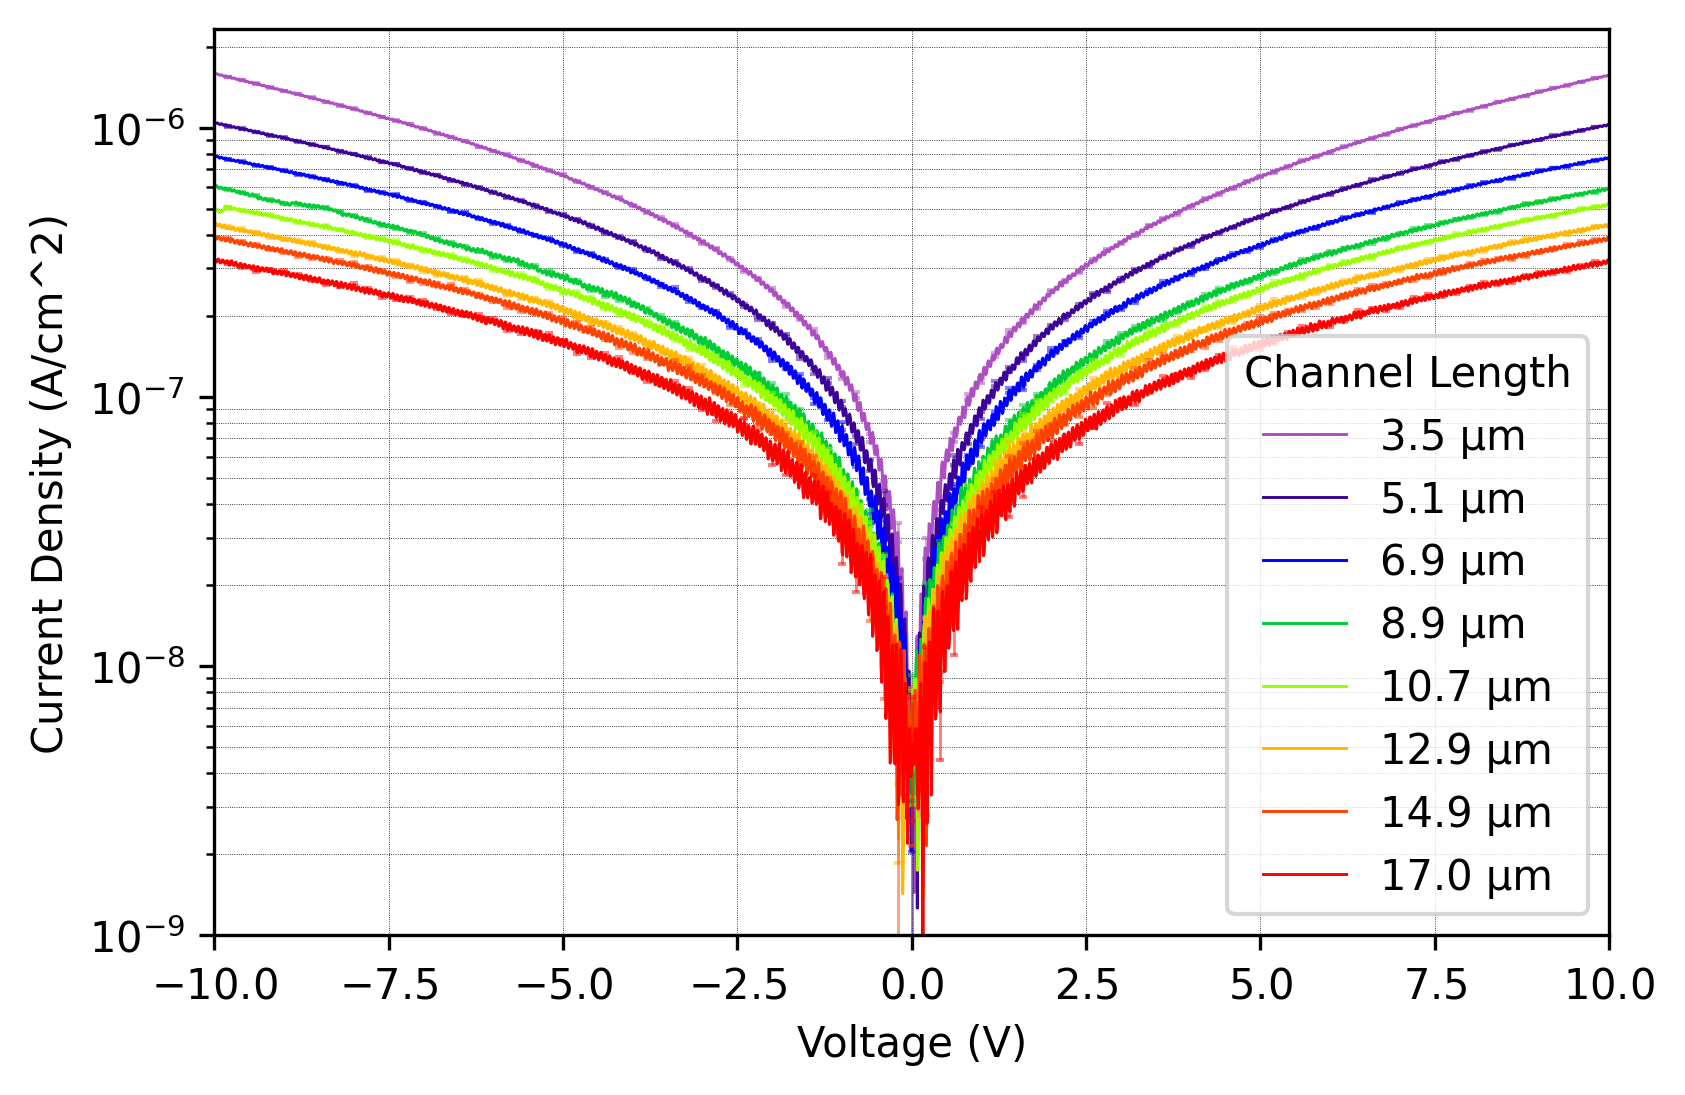
\includegraphics[width=0.97\textwidth]{Chapter6/Figs/Raster/Sample C 2019/10V_Current_Density_vs_Voltage_Temperature_21_log.png}
    \caption{A log-linear plot of the measured current density against applied voltage for all channel lengths at 21\si{\degreeCelsius} (sample C).}
    \label{appfig:current_density_21}
\end{figure}

\begin{figure}[h]
    \centering
    \includegraphics[width=0.97\textwidth]{Sample C 2019/10V_Current_Density_vs_Voltage_Temperature_50_log.png}
    \caption{A log-linear plot of the measured current density against applied voltage for all channel lengths at 50\si{\degreeCelsius} (sample C).}
    \label{appfig:current_density_50}
\end{figure}
\begin{figure}[h]
    \centering
    \includegraphics[width=0.97\textwidth]{Sample C 2019/10V_Current_Density_vs_Voltage_Temperature_100_log.png}
    \caption{A log-linear plot of the measured current density against applied voltage for all channel lengths at 100\si{\degreeCelsius} (sample C).}
    \label{appfig:current_density_100}
\end{figure}
\begin{figure}[h]
    \centering
    \includegraphics[width=0.97\textwidth]{Sample C 2019/10V_Current_Density_vs_Voltage_Temperature_150_log.png}
    \caption{A log-linear plot of the measured current density against applied voltage for all channel lengths at 150\si{\degreeCelsius} (sample C).}
    \label{appfig:current_density_150}
\end{figure}
\begin{figure}[h]
    \centering
    \includegraphics[width=0.97\textwidth]{Sample C 2019/10V_Current_Density_vs_Voltage_Temperature_200_log.png}
    \caption{A log-linear plot of the measured current density against applied voltage for all channel lengths at 200\si{\degreeCelsius} (sample C).}
    \label{appfig:current_density_200}
\end{figure}
\begin{figure}[h]
    \centering
    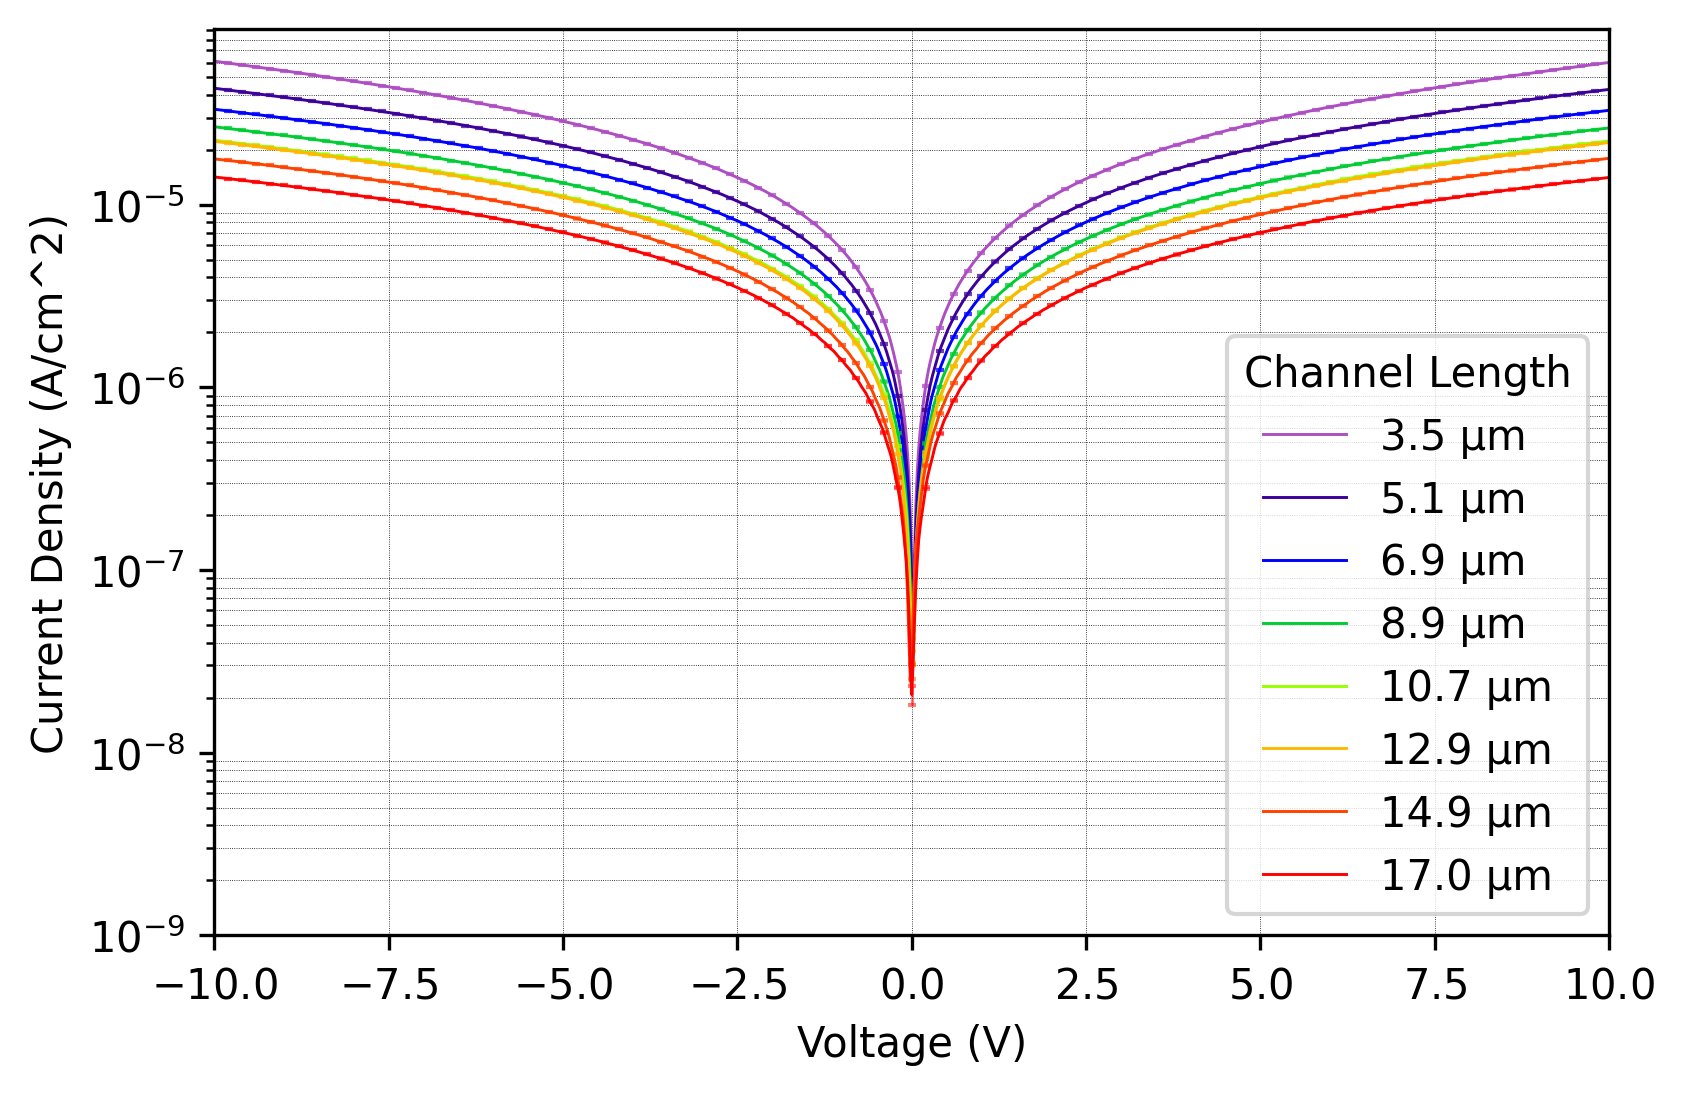
\includegraphics[width=0.97\textwidth]{Chapter6/Figs/Raster/Sample C 2019/10V_Current_Density_vs_Voltage_Temperature_250_log.png}
    \caption{A log-linear plot of the measured current density against applied voltage for all channel lengths at 250\si{\degreeCelsius} (sample C).}
    \label{appfig:current_density_250}
\end{figure}
\begin{figure}[h]
    \centering
    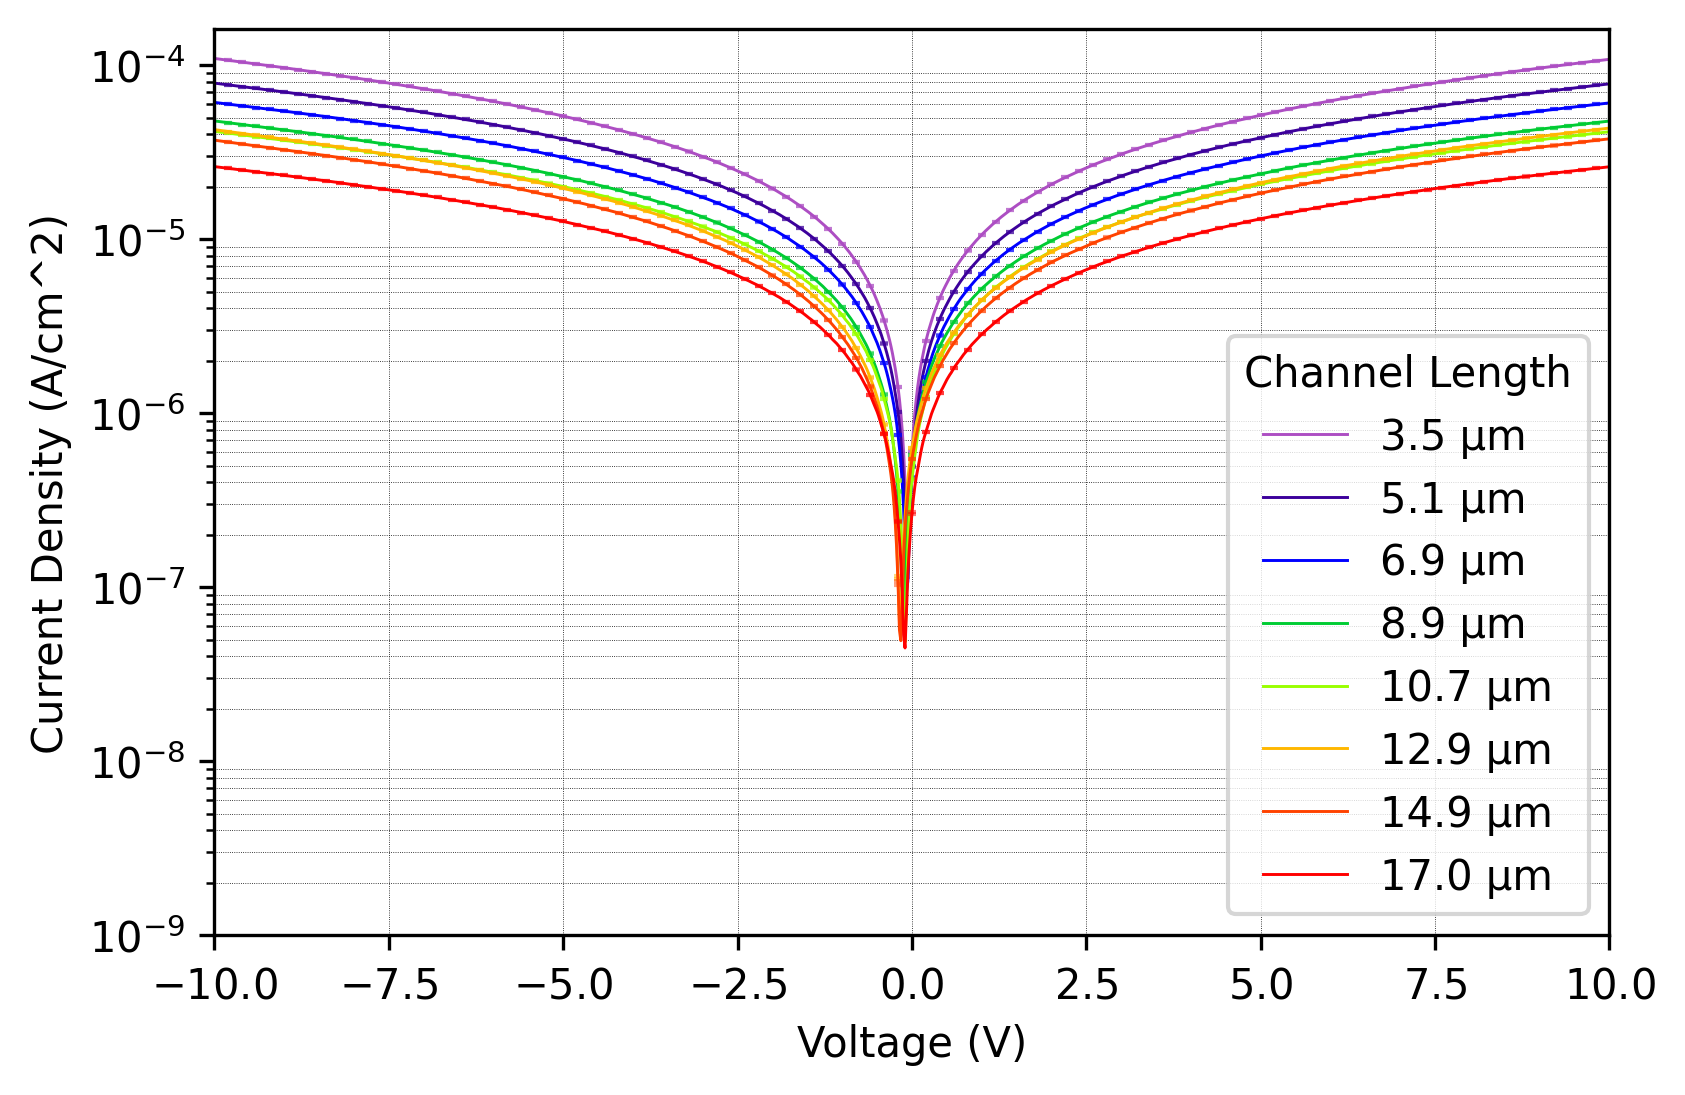
\includegraphics[width=0.97\textwidth]{Chapter6/Figs/Raster/Sample C 2019/10V_Current_Density_vs_Voltage_Temperature_300_log.png}
    \caption{A log-linear plot of the measured current density against applied voltage for all channel lengths at 300\si{\degreeCelsius} (sample C).}
    \label{appfig:current_density_300}
\end{figure}

\subsection{Sample D: 10 \si{\volt} range}
\label{app:J_V_sample_D_10V}

\begin{figure}[h]
    \centering
    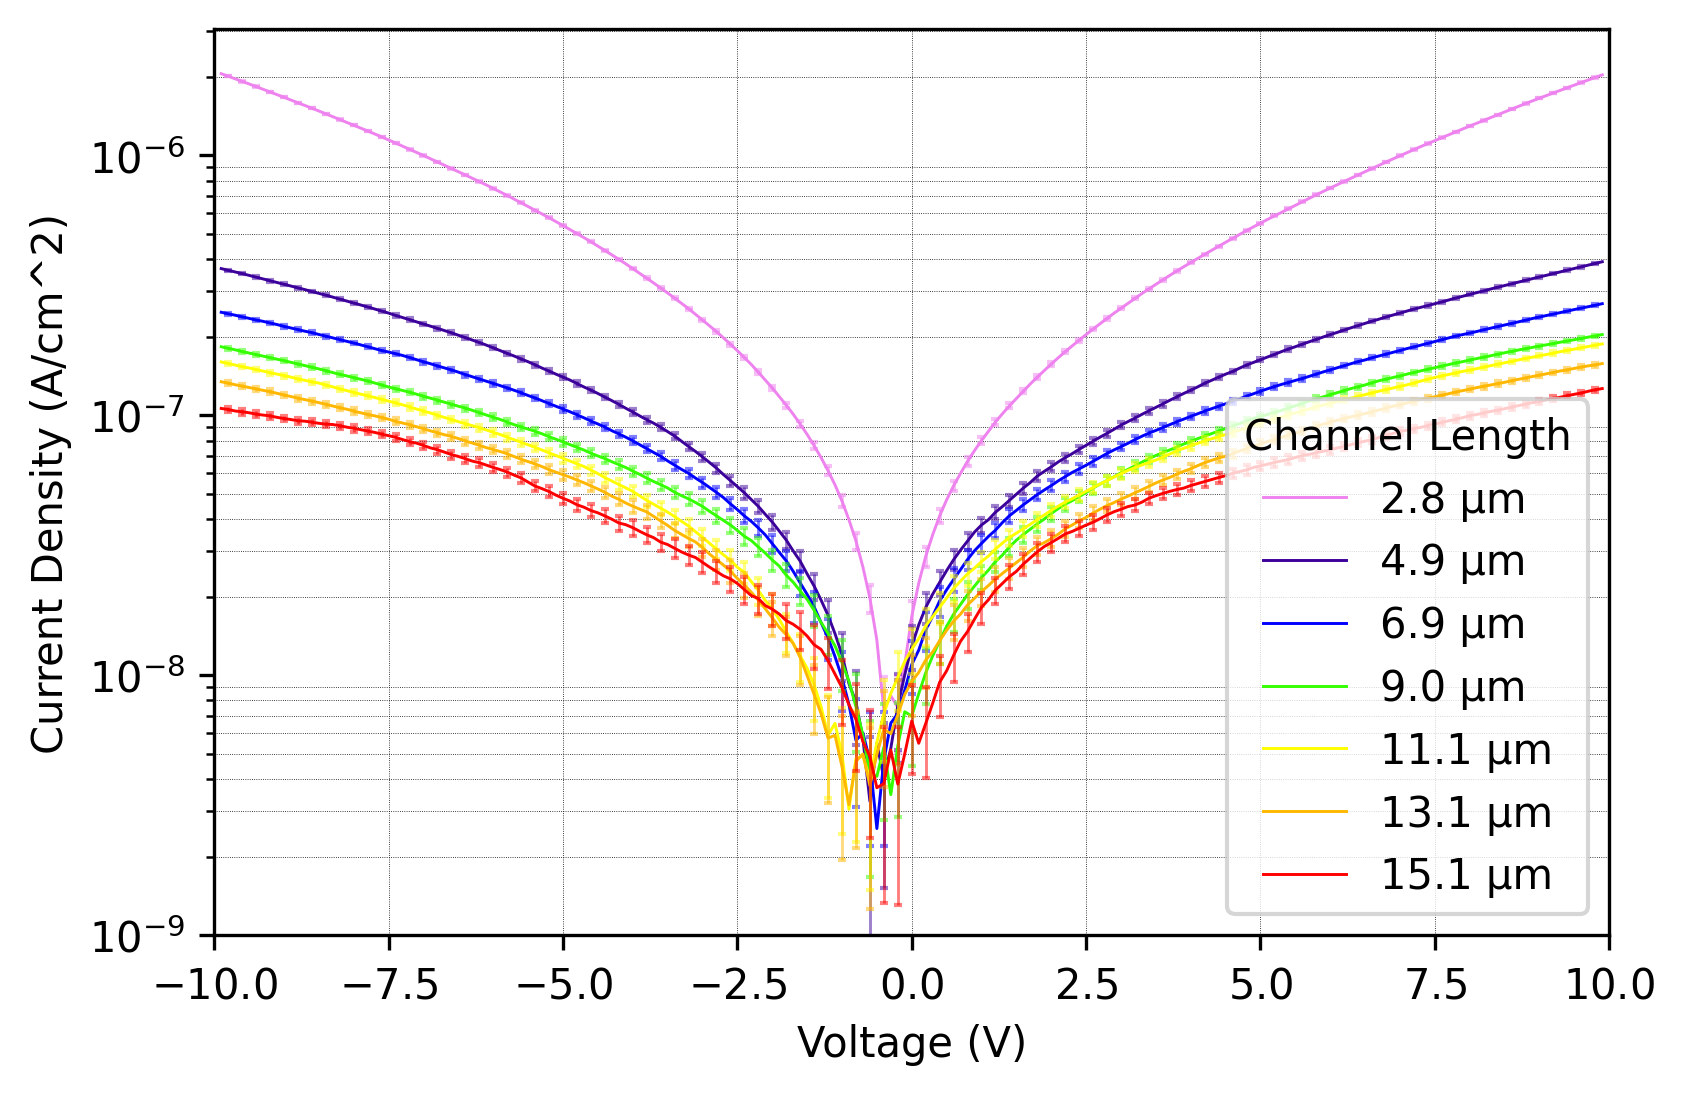
\includegraphics[width=0.97\textwidth]{Chapter6/Figs/Raster/Sample D 2019/10V_Current_Density_vs_Voltage_Temperature_21_log.png}
    \caption{A log-linear plot of the measured current density against applied voltage for all channel lengths at 21\si{\degreeCelsius} (sample D).}
    \label{appfig:10V_D_current_density_21}
\end{figure}
\begin{figure}[h]
    \centering
    \includegraphics[width=0.97\textwidth]{Sample D 2019/10V_Current_Density_vs_Voltage_Temperature_50_log.png}
    \caption{A log-linear plot of the measured current density against applied voltage for all channel lengths at 50\si{\degreeCelsius} (sample D).}
    \label{appfig:10V_D_current_density_50}
\end{figure}
\begin{figure}[h]
    \centering
    \includegraphics[width=0.97\textwidth]{Sample D 2019/10V_Current_Density_vs_Voltage_Temperature_100_log.png}
    \caption{A log-linear plot of the measured current density against applied voltage for all channel lengths at 100\si{\degreeCelsius} (sample D).}
    \label{appfig:10V_D_current_density_100}
\end{figure}
\begin{figure}[h]
    \centering
    \includegraphics[width=0.97\textwidth]{Sample D 2019/10V_Current_Density_vs_Voltage_Temperature_150_log.png}
    \caption{A log-linear plot of the measured current density against applied voltage for all channel lengths at 150\si{\degreeCelsius} (sample D).}
    \label{appfig:10V_D_current_density_150}
\end{figure}
\begin{figure}[h]
    \centering
    \includegraphics[width=0.97\textwidth]{Sample D 2019/10V_Current_Density_vs_Voltage_Temperature_200_log.png}
    \caption{A log-linear plot of the measured current density against applied voltage for all channel lengths at 200\si{\degreeCelsius} (sample D).}
    \label{appfig:10V_D_current_density_200}
\end{figure}
\begin{figure}[h]
    \centering
    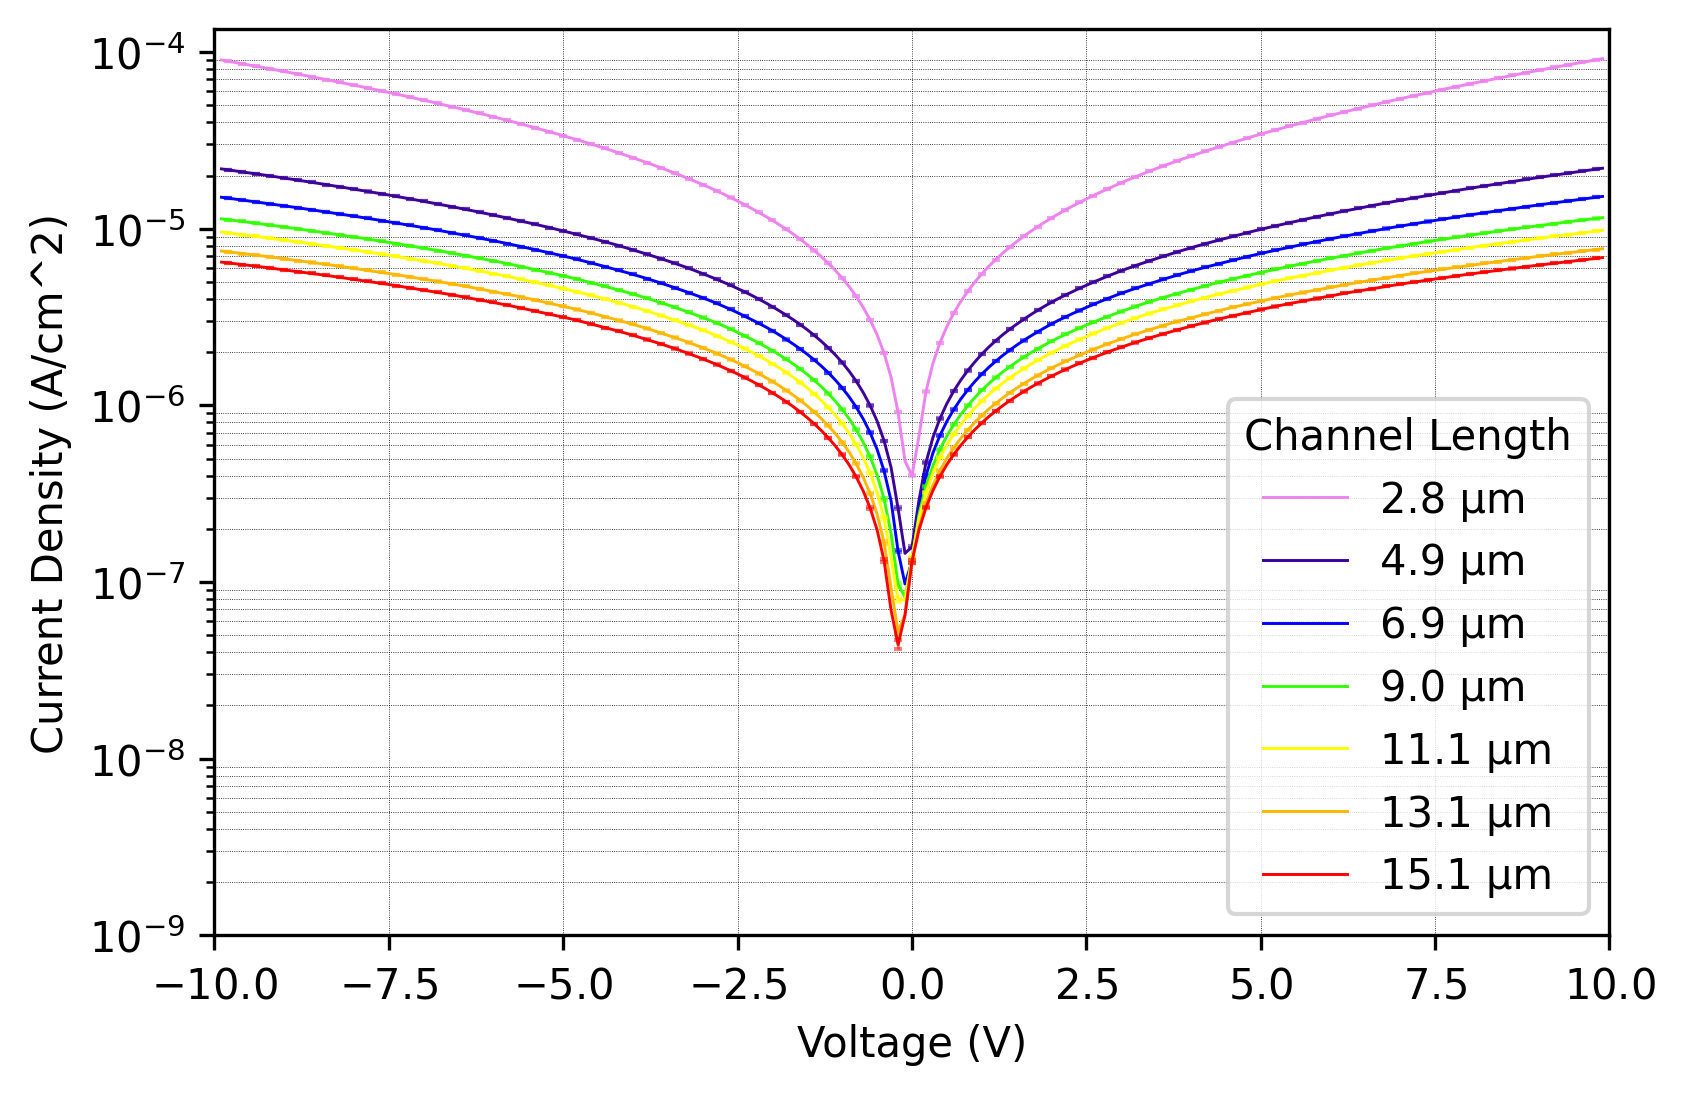
\includegraphics[width=0.97\textwidth]{Chapter6/Figs/Raster/Sample D 2019/10V_Current_Density_vs_Voltage_Temperature_250_log.png}
    \caption{A log-linear plot of the measured current density against applied voltage for all channel lengths at 250\si{\degreeCelsius} (sample D).}
    \label{appfig:10V_D_current_density_250}
\end{figure}
\begin{figure}[h]
    \centering
    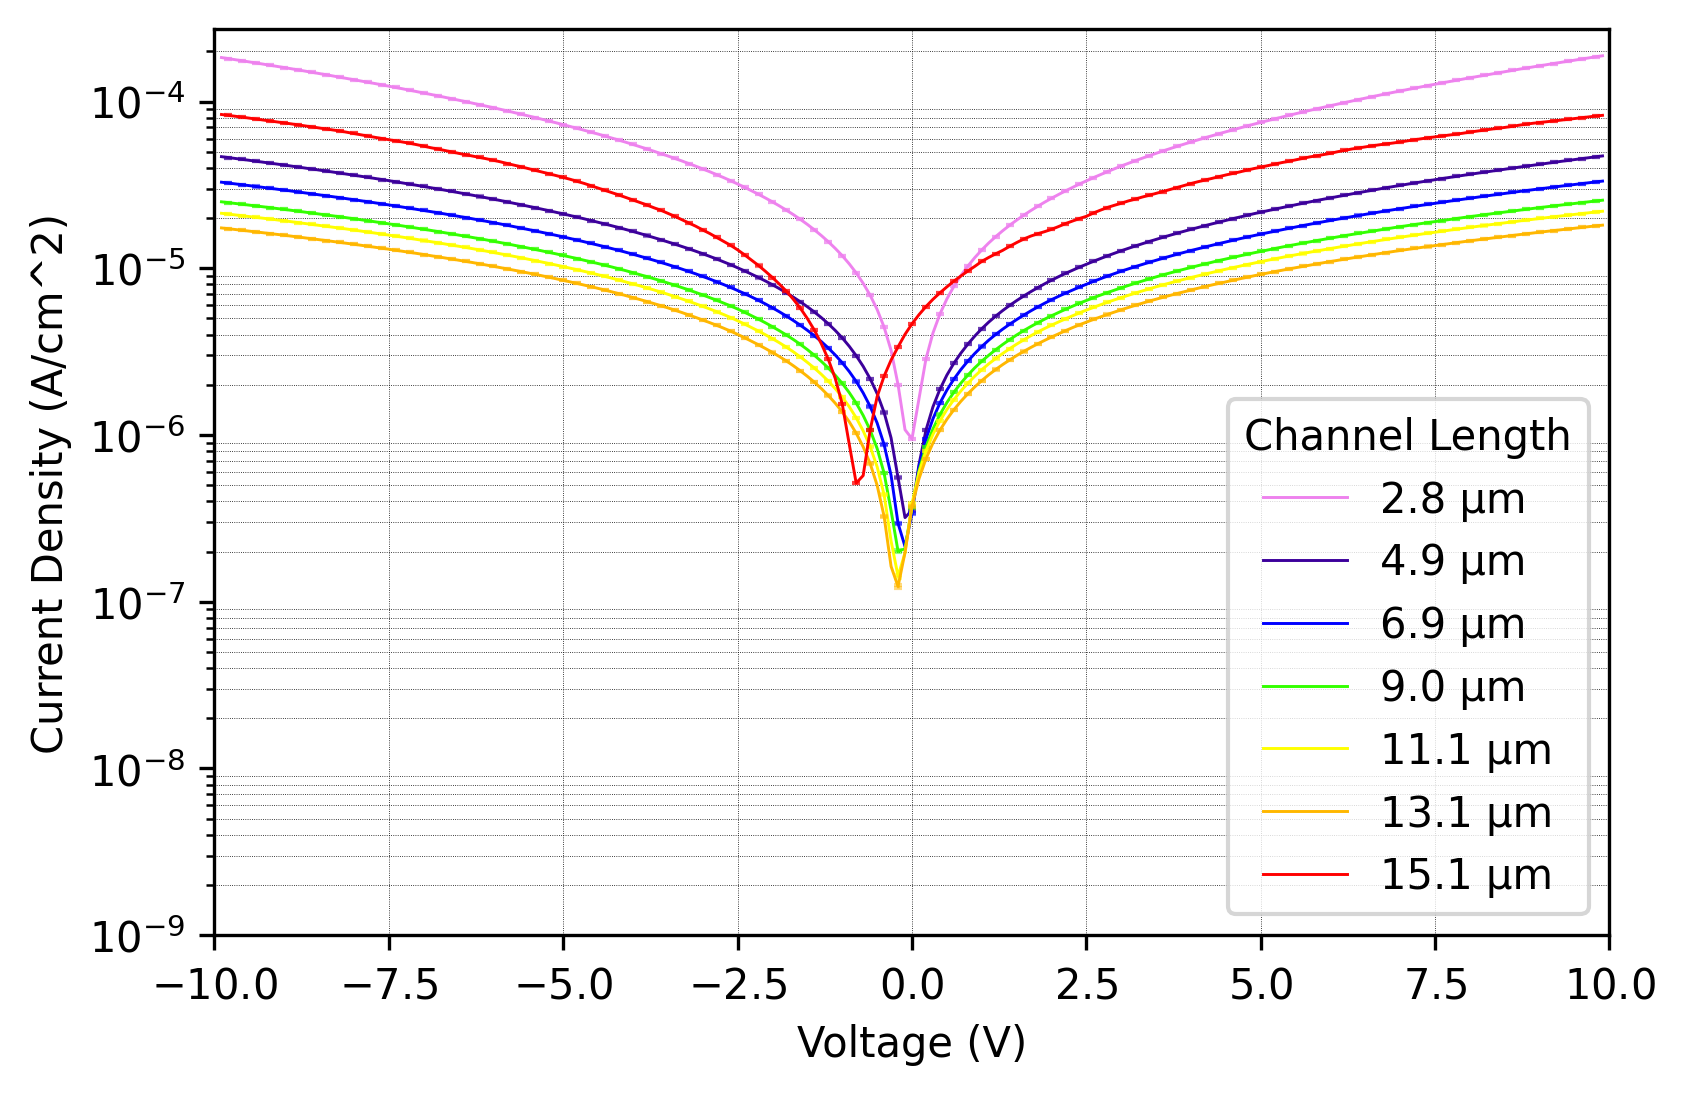
\includegraphics[width=0.97\textwidth]{Chapter6/Figs/Raster/Sample D 2019/10V_Current_Density_vs_Voltage_Temperature_300_log.png}
    \caption{A log-linear plot of the measured current density against applied voltage for all channel lengths at 300\si{\degreeCelsius} (sample D).}
    \label{appfig:10V_D_current_density_300}
\end{figure}

\subsection{Sample D: 50 \si{\volt} range}

\label{app:J_V_sample_D_10V}
\begin{figure}[h]
    \centering
    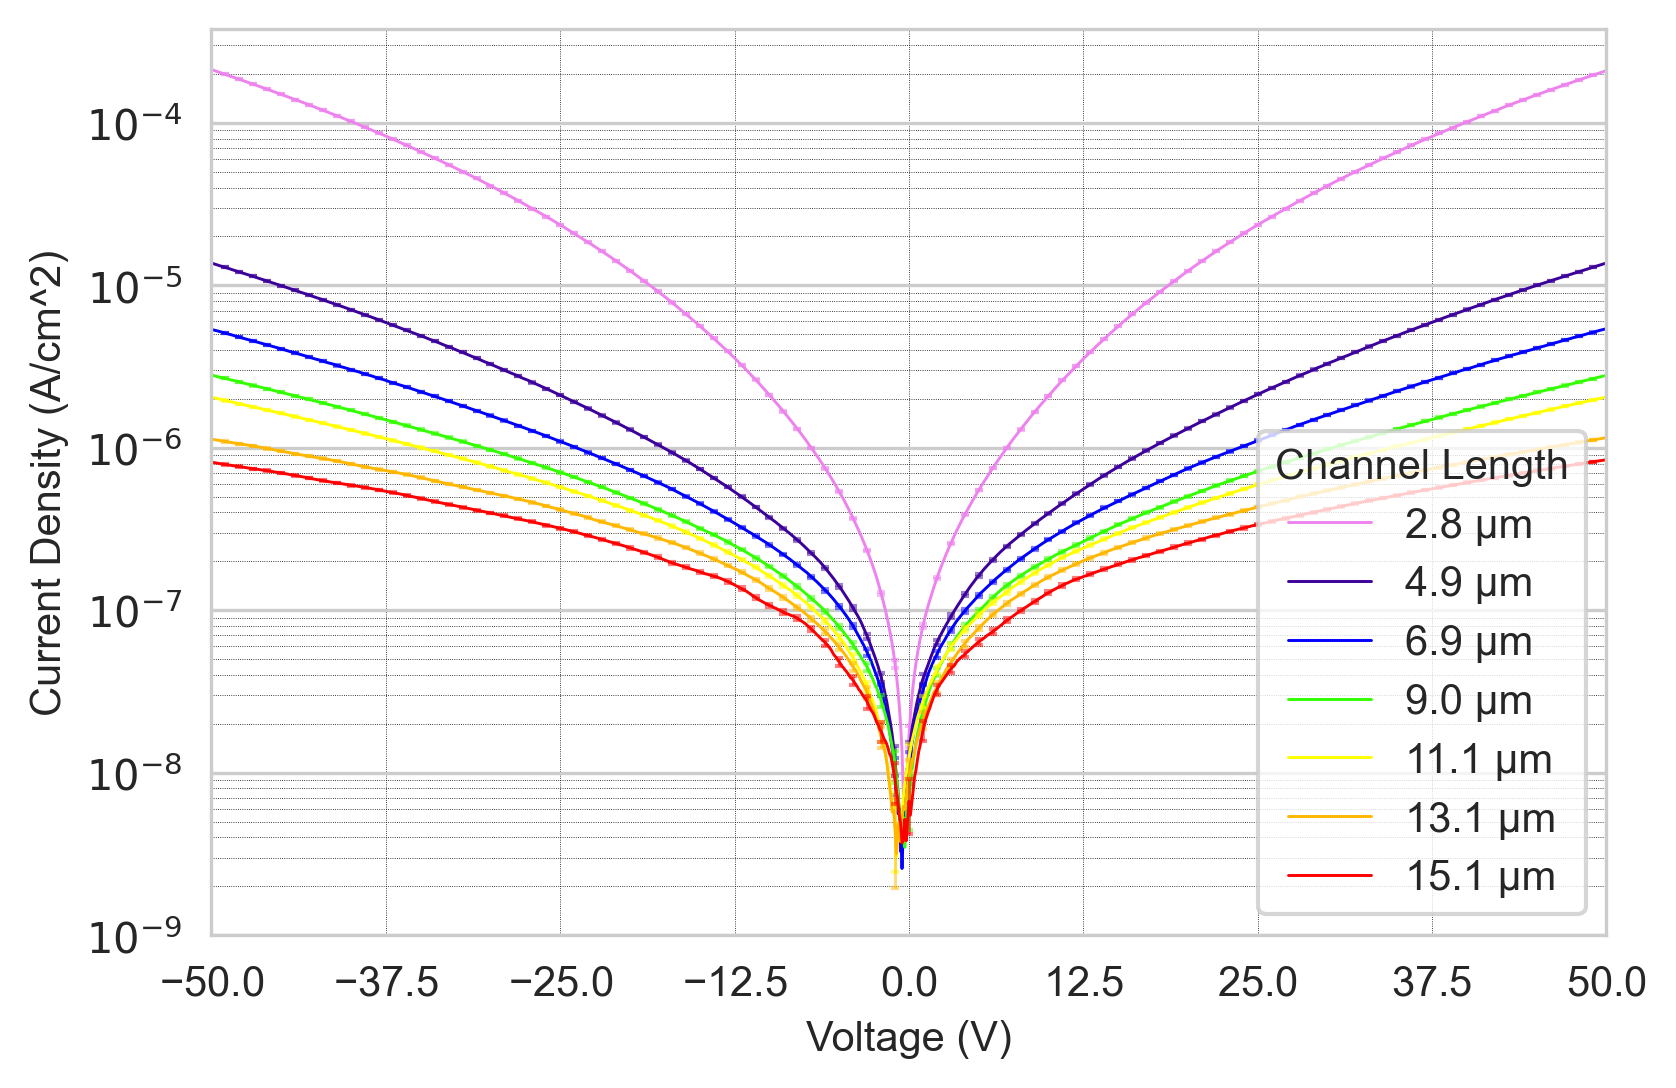
\includegraphics[width=0.97\textwidth]{Chapter6/Figs/Raster/Sample D 2019/50V_Current_Density_vs_Voltage_Temperature_21_log.png}
    \caption{A log-linear plot of the measured current density against applied voltage for all channel lengths at 21\si{\degreeCelsius} (sample D).}
    \label{appfig:D_current_density_21}
\end{figure}
\begin{figure}[h]
    \centering
    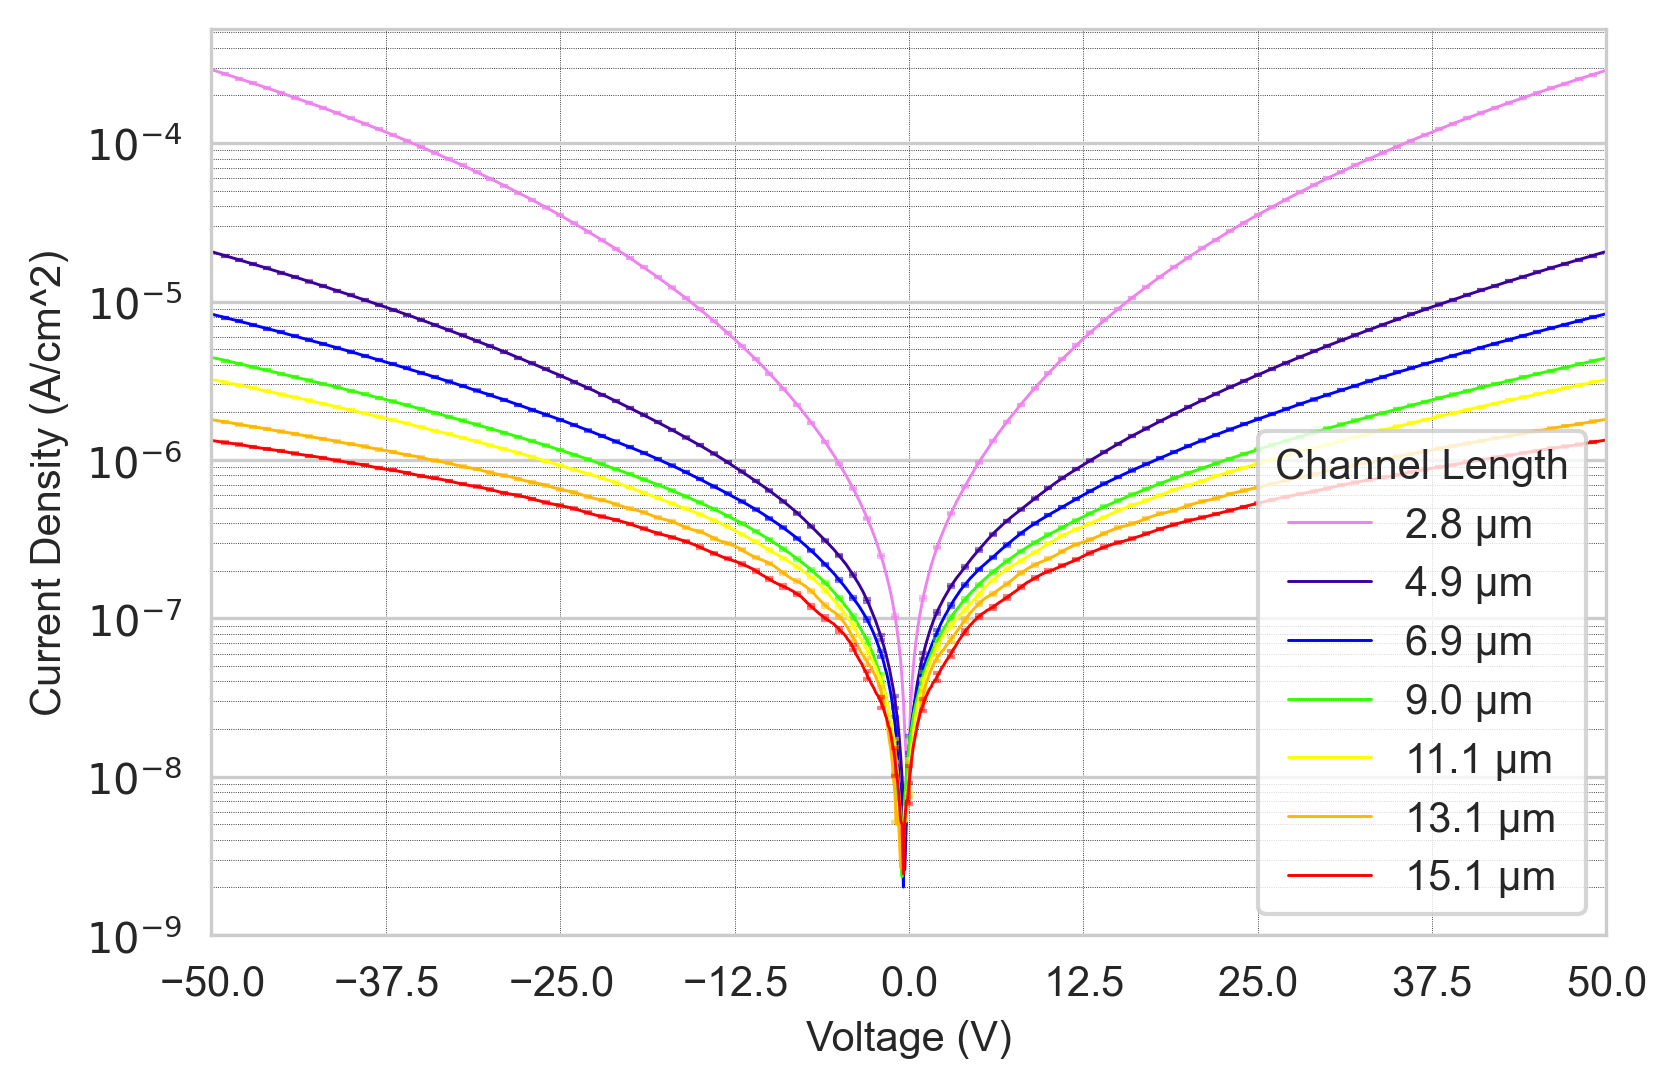
\includegraphics[width=0.97\textwidth]{Sample D 2019/50V_Current_Density_vs_Voltage_Temperature_50_log.png}
    \caption{A log-linear plot of the measured current density against applied voltage for all channel lengths at 50\si{\degreeCelsius} (sample D).}
    \label{appfig:D_current_density_50}
\end{figure}
\begin{figure}[h]
    \centering
    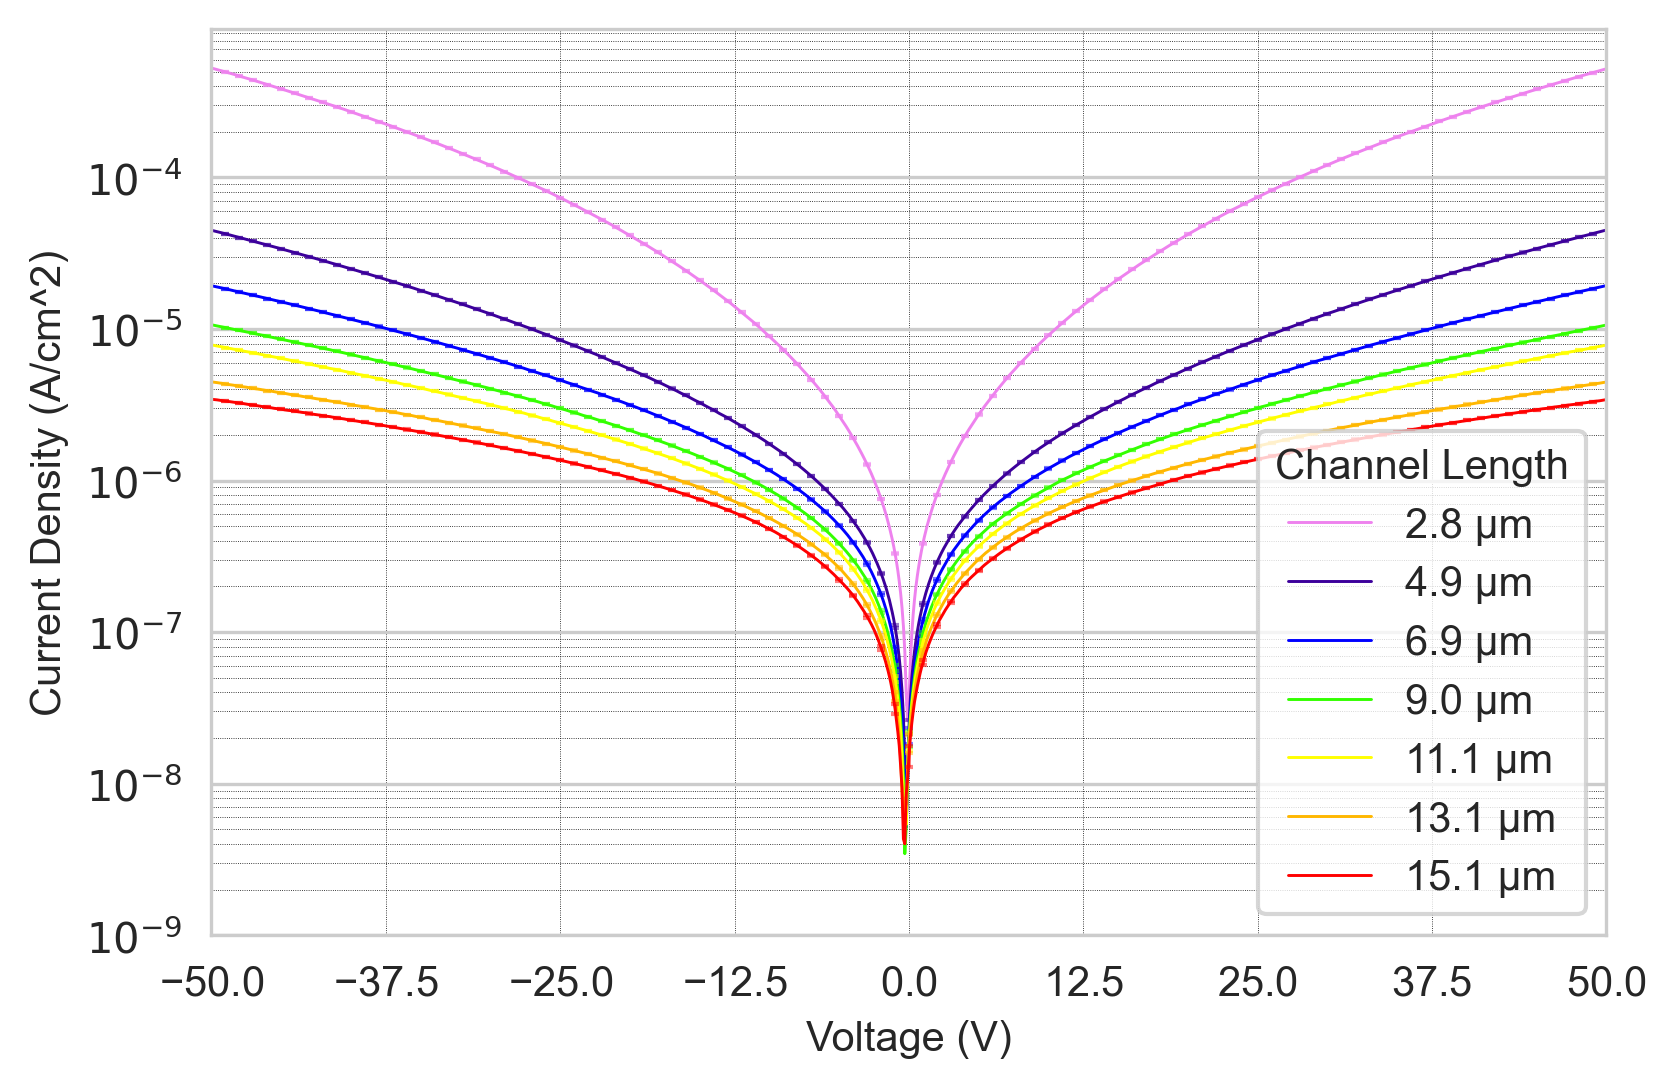
\includegraphics[width=0.97\textwidth]{Sample D 2019/50V_Current_Density_vs_Voltage_Temperature_100_log.png}
    \caption{A log-linear plot of the measured current density against applied voltage for all channel lengths at 100\si{\degreeCelsius} (sample D).}
    \label{appfig:D_current_density_100}
\end{figure}
\begin{figure}[h]
    \centering
    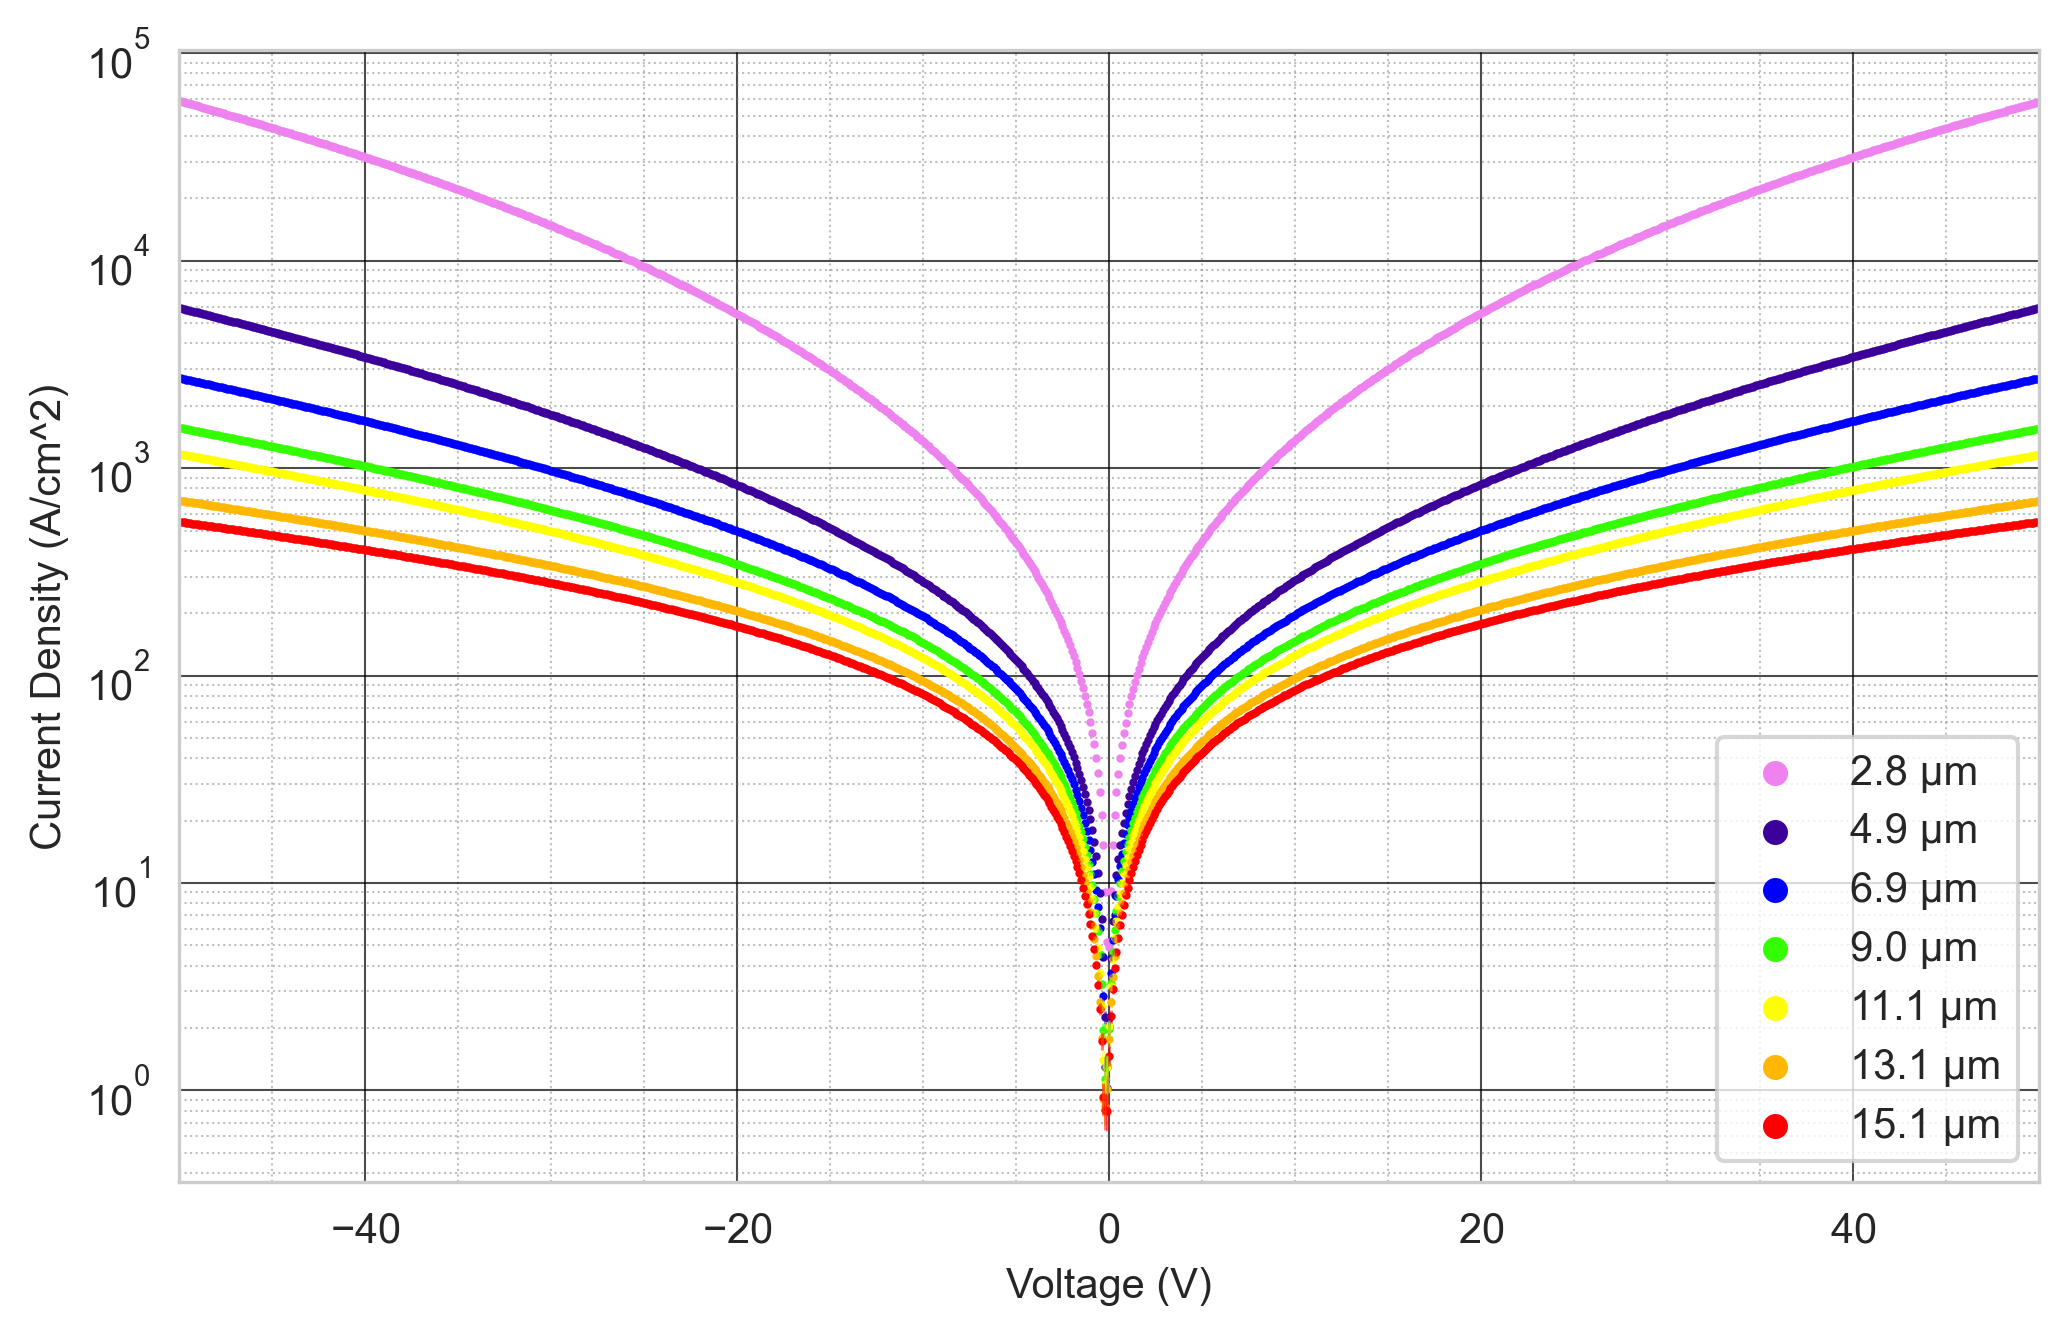
\includegraphics[width=0.97\textwidth]{Sample D 2019/50V_Current_Density_vs_Voltage_Temperature_150_log.png}
    \caption{A log-linear plot of the measured current density against applied voltage for all channel lengths at 150\si{\degreeCelsius} (sample D).}
    \label{appfig:D_current_density_150}
\end{figure}
\begin{figure}[h]
    \centering
    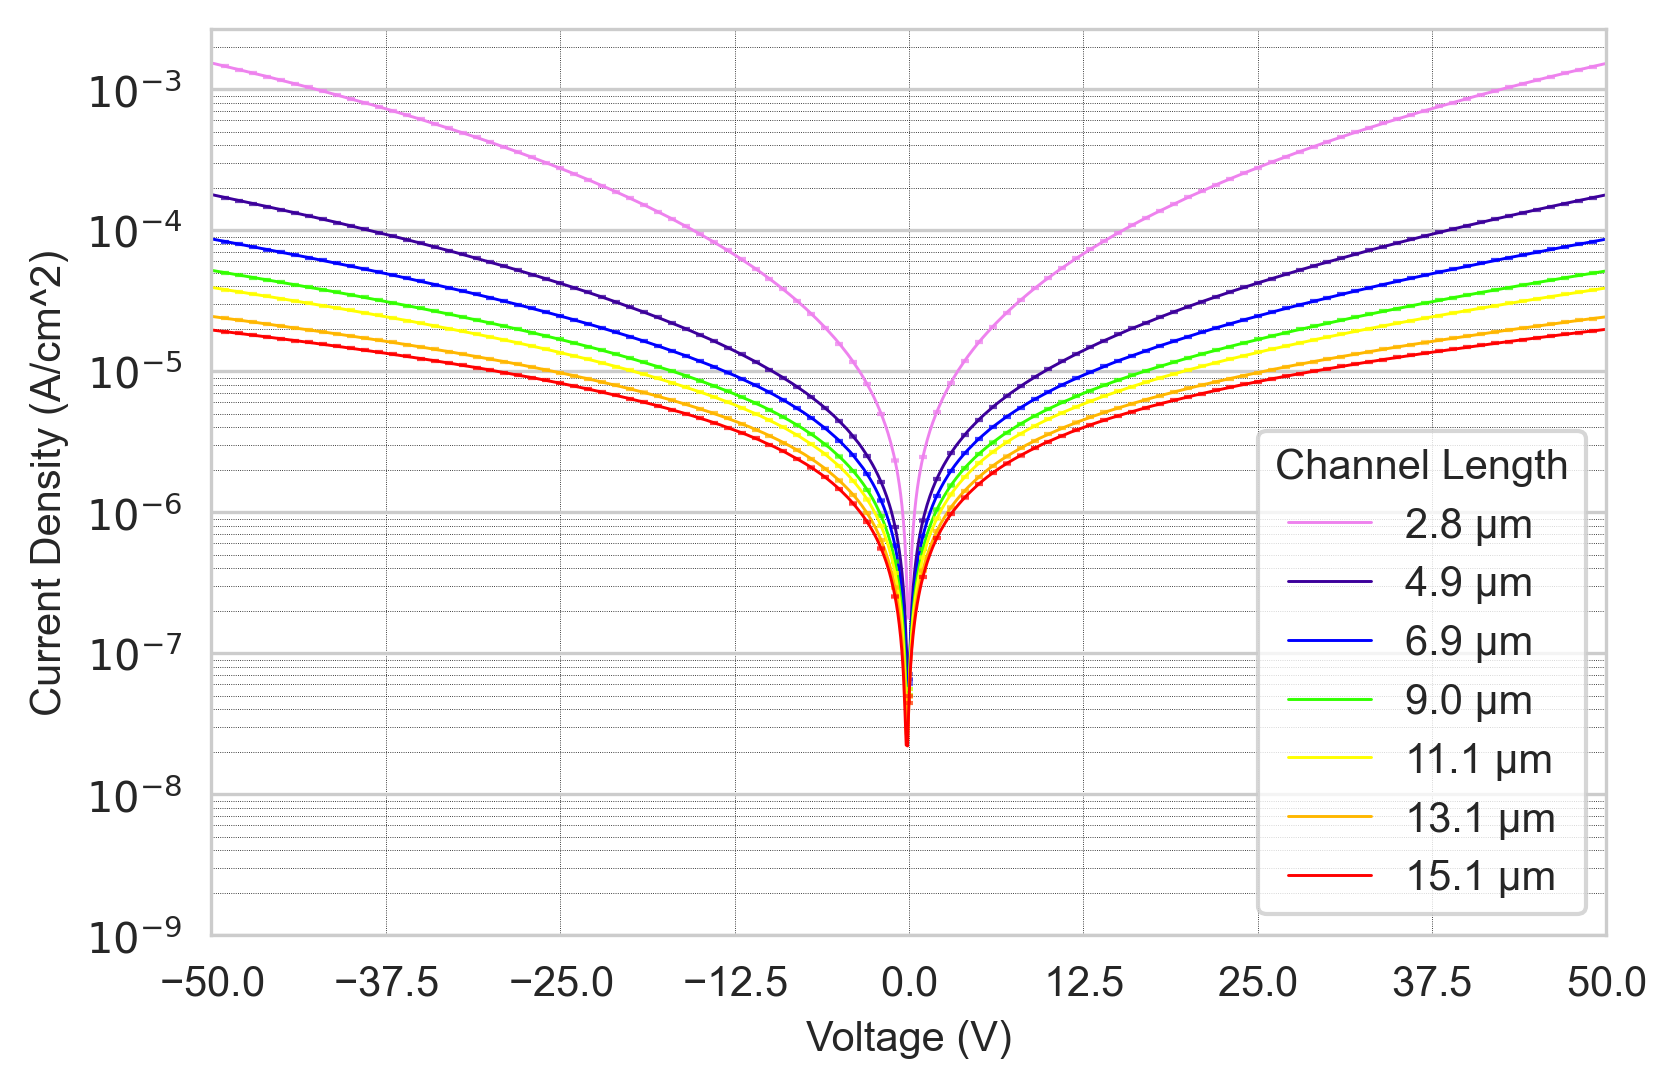
\includegraphics[width=0.97\textwidth]{Sample D 2019/50V_Current_Density_vs_Voltage_Temperature_200_log.png}
    \caption{A log-linear plot of the measured current density against applied voltage for all channel lengths at 200\si{\degreeCelsius} (sample D).}
    \label{appfig:D_current_density_200}
\end{figure}
\begin{figure}[h]
    \centering
    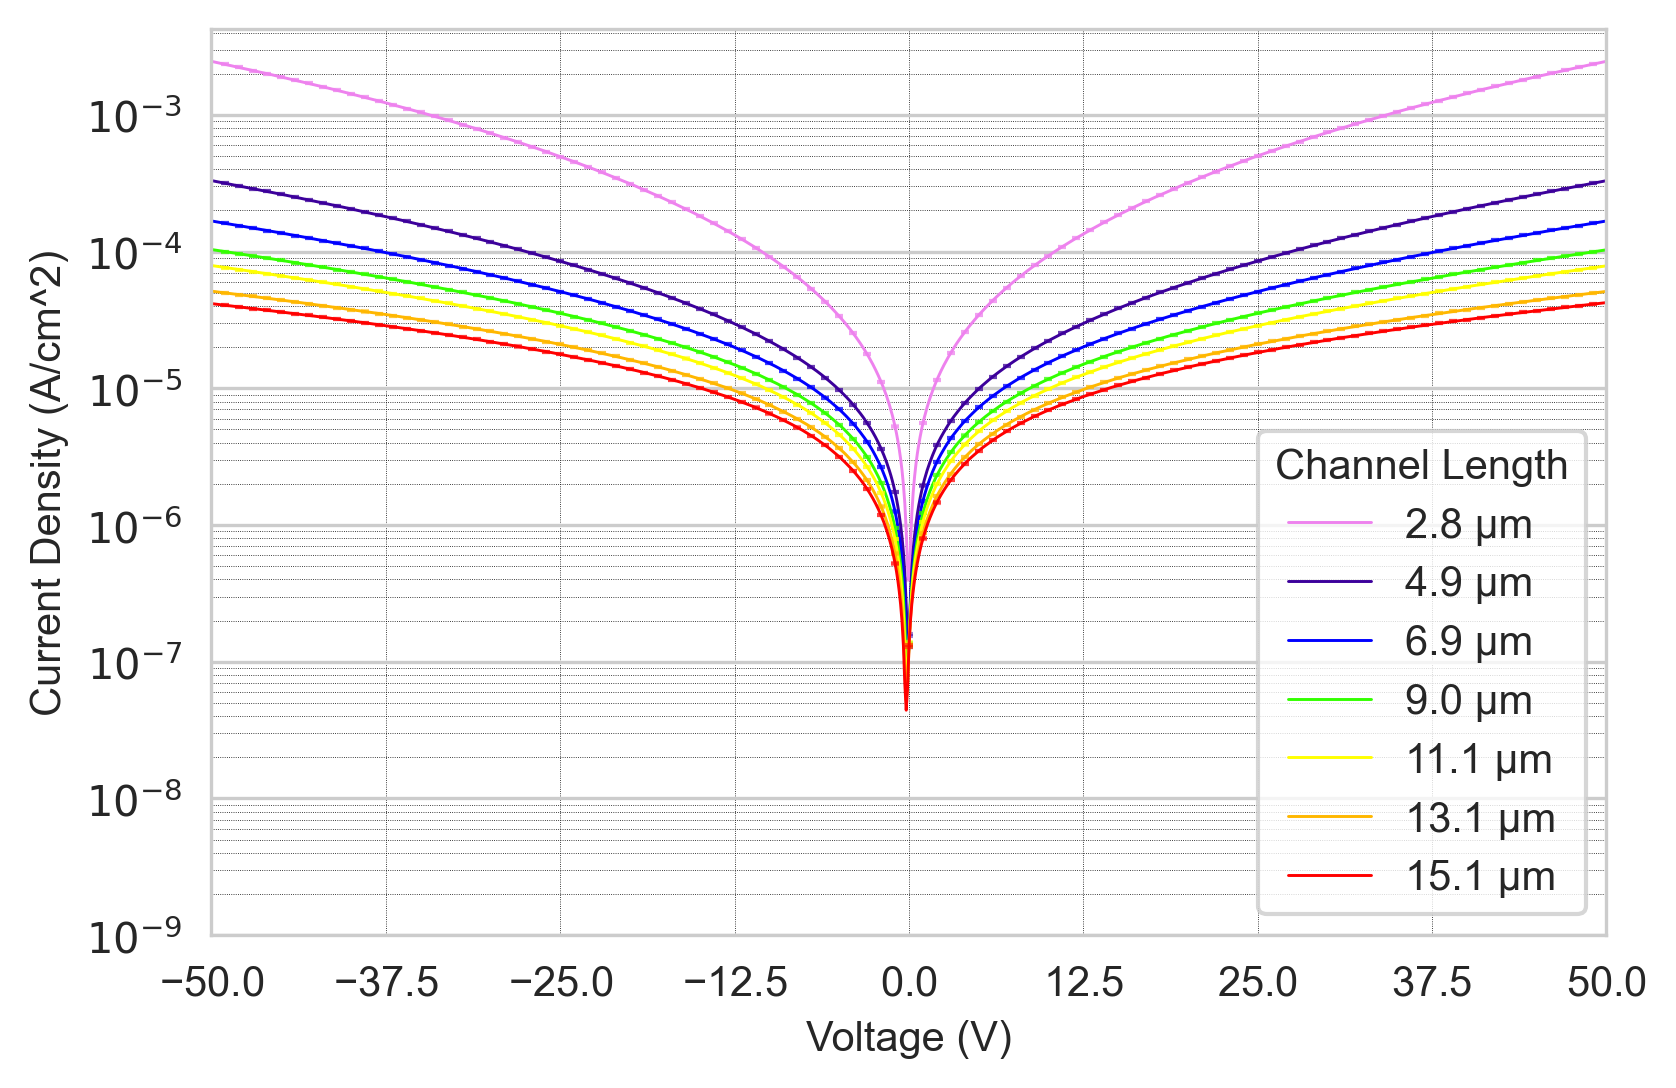
\includegraphics[width=0.97\textwidth]{Sample D 2019/50V_Current_Density_vs_Voltage_Temperature_250_log.png}
    \caption{A log-linear plot of the measured current density against applied voltage for all channel lengths at 250\si{\degreeCelsius} (sample D).}
    \label{appfig:D_current_density_250}
\end{figure}
\begin{figure}[h]
    \centering
    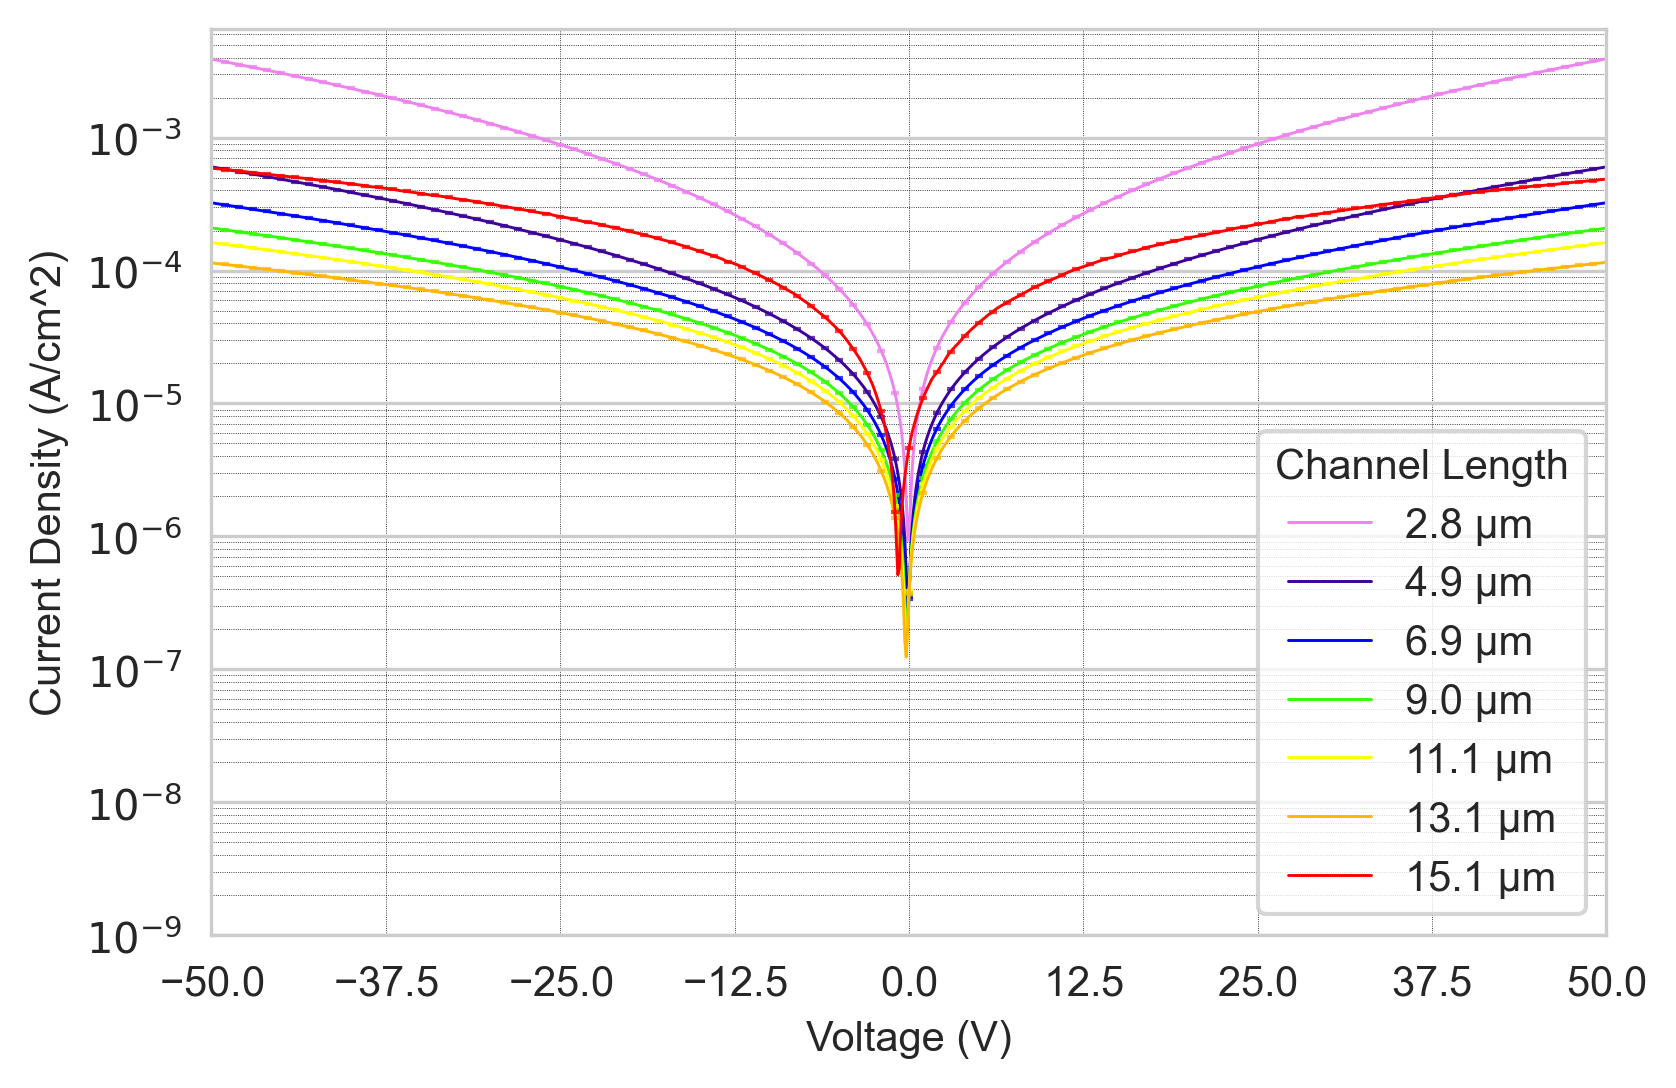
\includegraphics[width=0.97\textwidth]{Sample D 2019/50V_Current_Density_vs_Voltage_Temperature_300_log.png}
    \caption{A log-linear plot of the measured current density against applied voltage for all channel lengths at 300\si{\degreeCelsius} (sample D).}
    \label{appfig:D_current_density_300}
\end{figure}

\section{LTLM I-V, samples C and D}
\label{app:LTLM_I_V_data}

For reference, error bars of 2 \si{\pico\ampere} are plotted on a limited bias range of $\pm1$ \si{\volt} in figure \ref{appfig:1V_C_current_voltage_21}.

\begin{figure}[h]
    \centering
    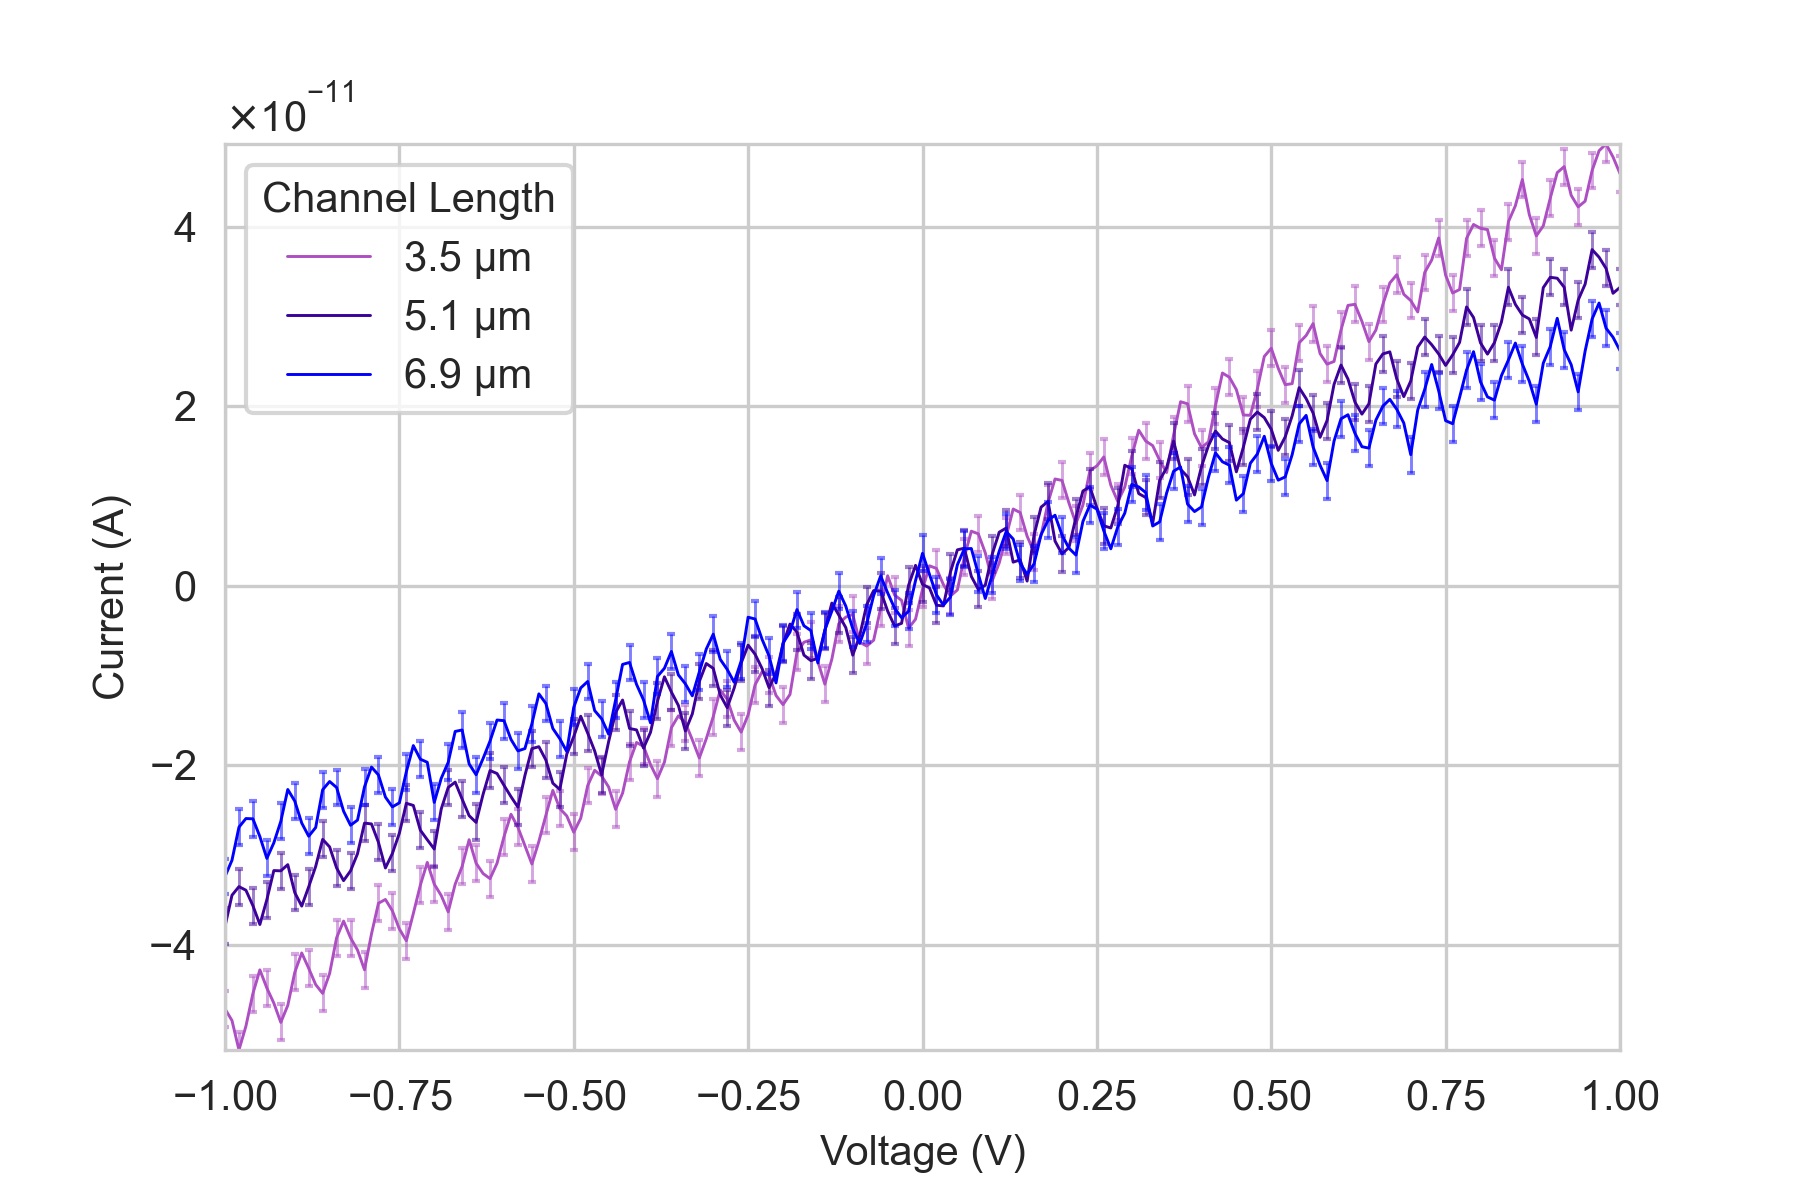
\includegraphics[width=0.97\textwidth]{Appendix1/1V IV characteristics at 21 C.png}
    \caption{A linear plot of the measured current against applied voltage for three channel lengths, $\pm1$ \si{\volt}, with 2 \si{\pico\ampere} error bars at 21\si{\degreeCelsius} (sample C).}
    \label{appfig:1V_C_current_voltage_21}
\end{figure}


\subsection{Sample C: 10 \si{\volt} range}
\label{app:I_V_sample_C}

\begin{figure}[h]
    \centering
    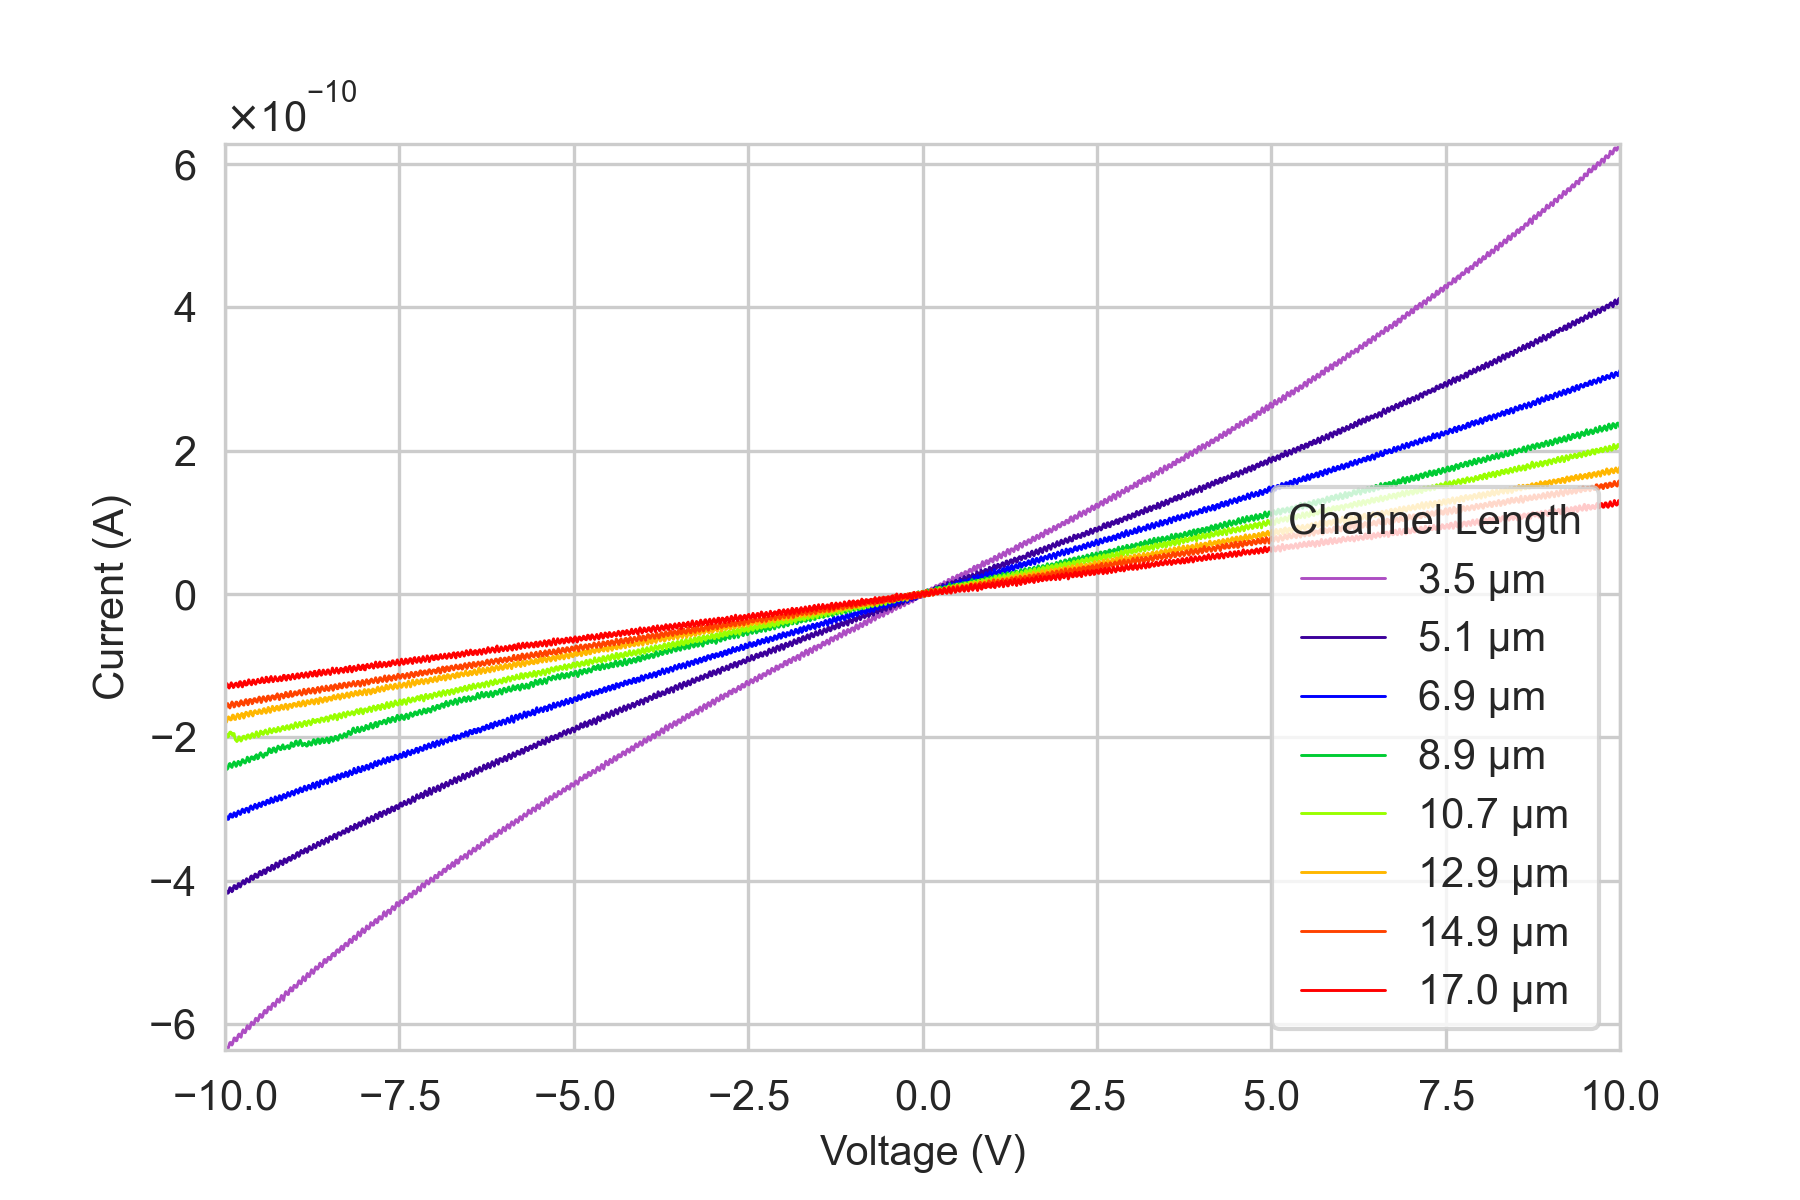
\includegraphics[width=0.97\textwidth]{Chapter6/Figs/Raster/Sample C 2019/IV/10V IV characteristics at 21 C.png}
    \caption{A linear plot of the measured current against applied voltage for all channel lengths at 21\si{\degreeCelsius} (sample C).}
    \label{appfig:C_current_voltage_21}
\end{figure}
\begin{figure}[h]
    \centering
    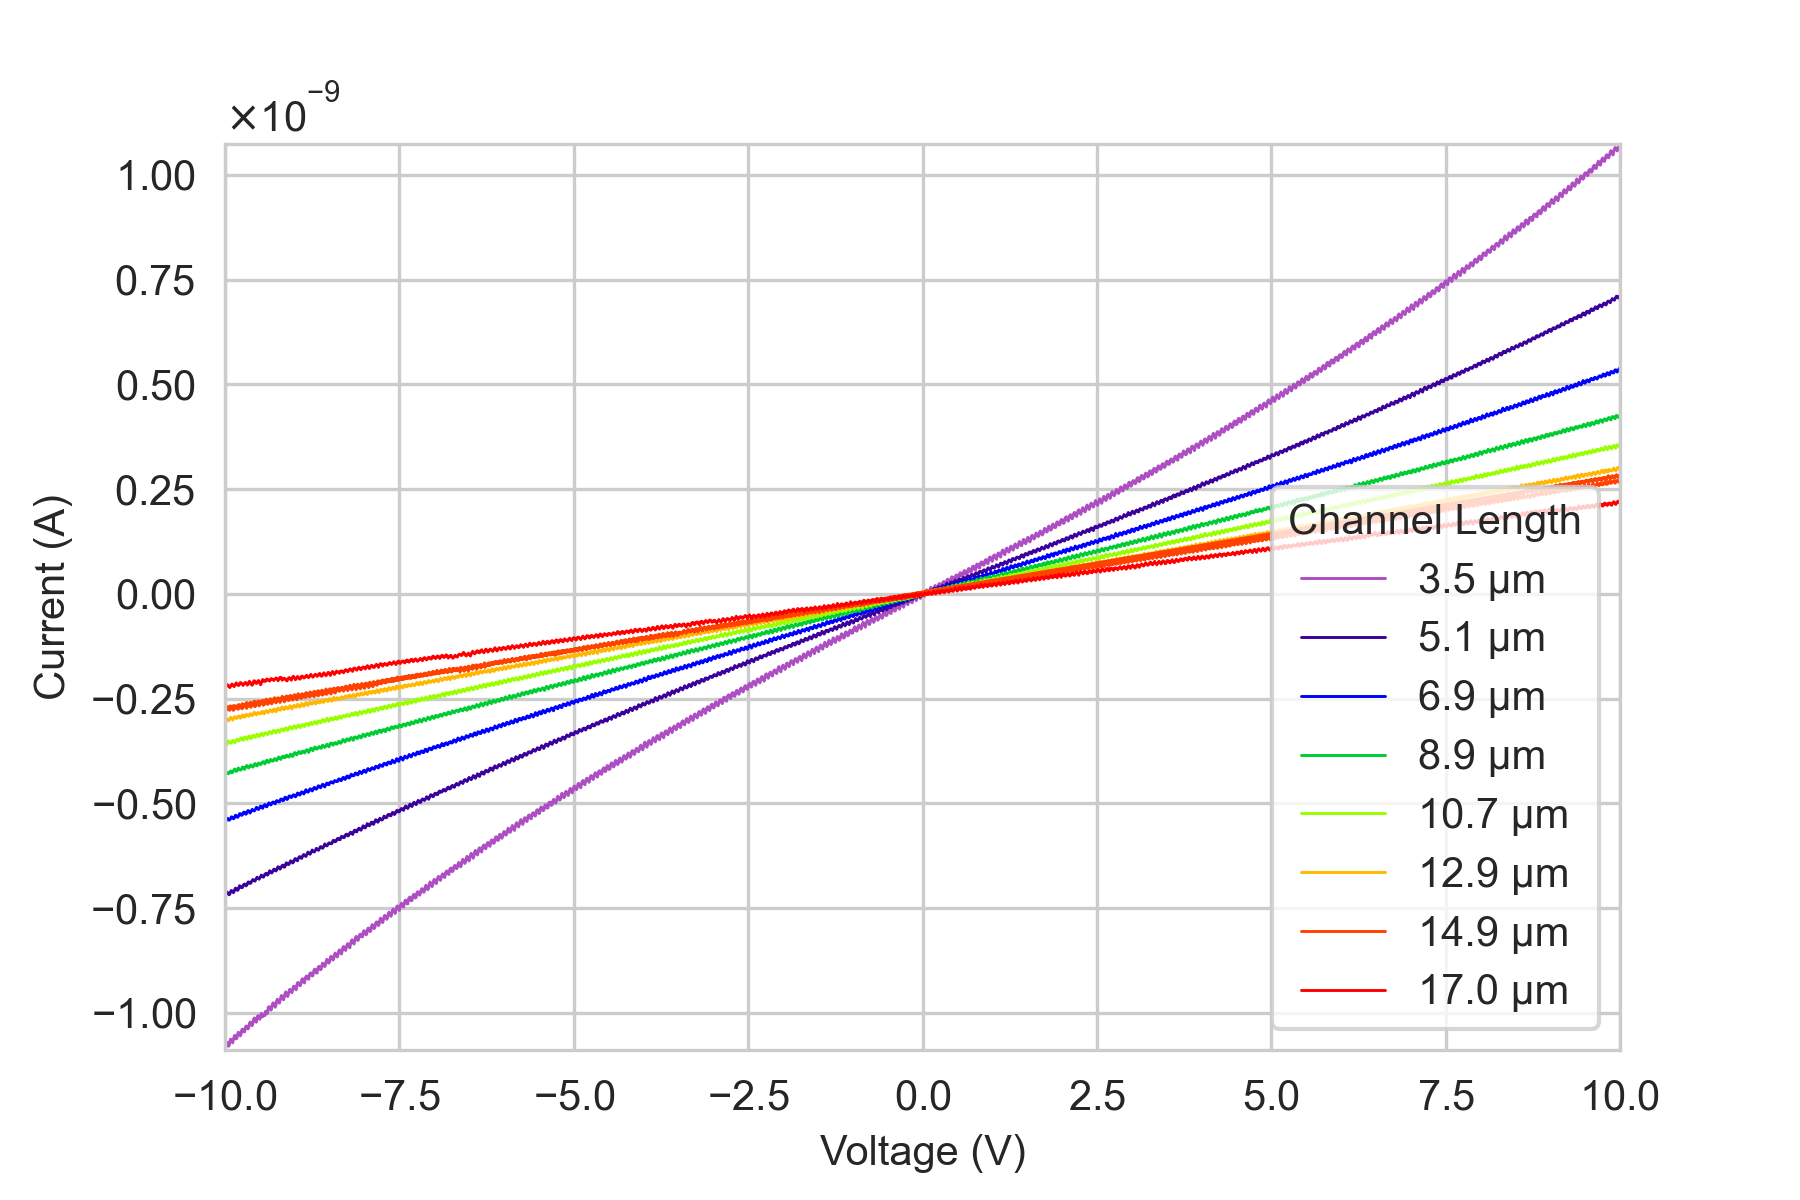
\includegraphics[width=0.97\textwidth]{Chapter6/Figs/Raster/Sample C 2019/IV/10V IV characteristics at 50 C.png}
    \caption{A linear plot of the measured current against applied voltage for all channel lengths at 50\si{\degreeCelsius} (sample C).}
    \label{appfig:C_current_voltage_50}
\end{figure}
\begin{figure}[h]
    \centering
    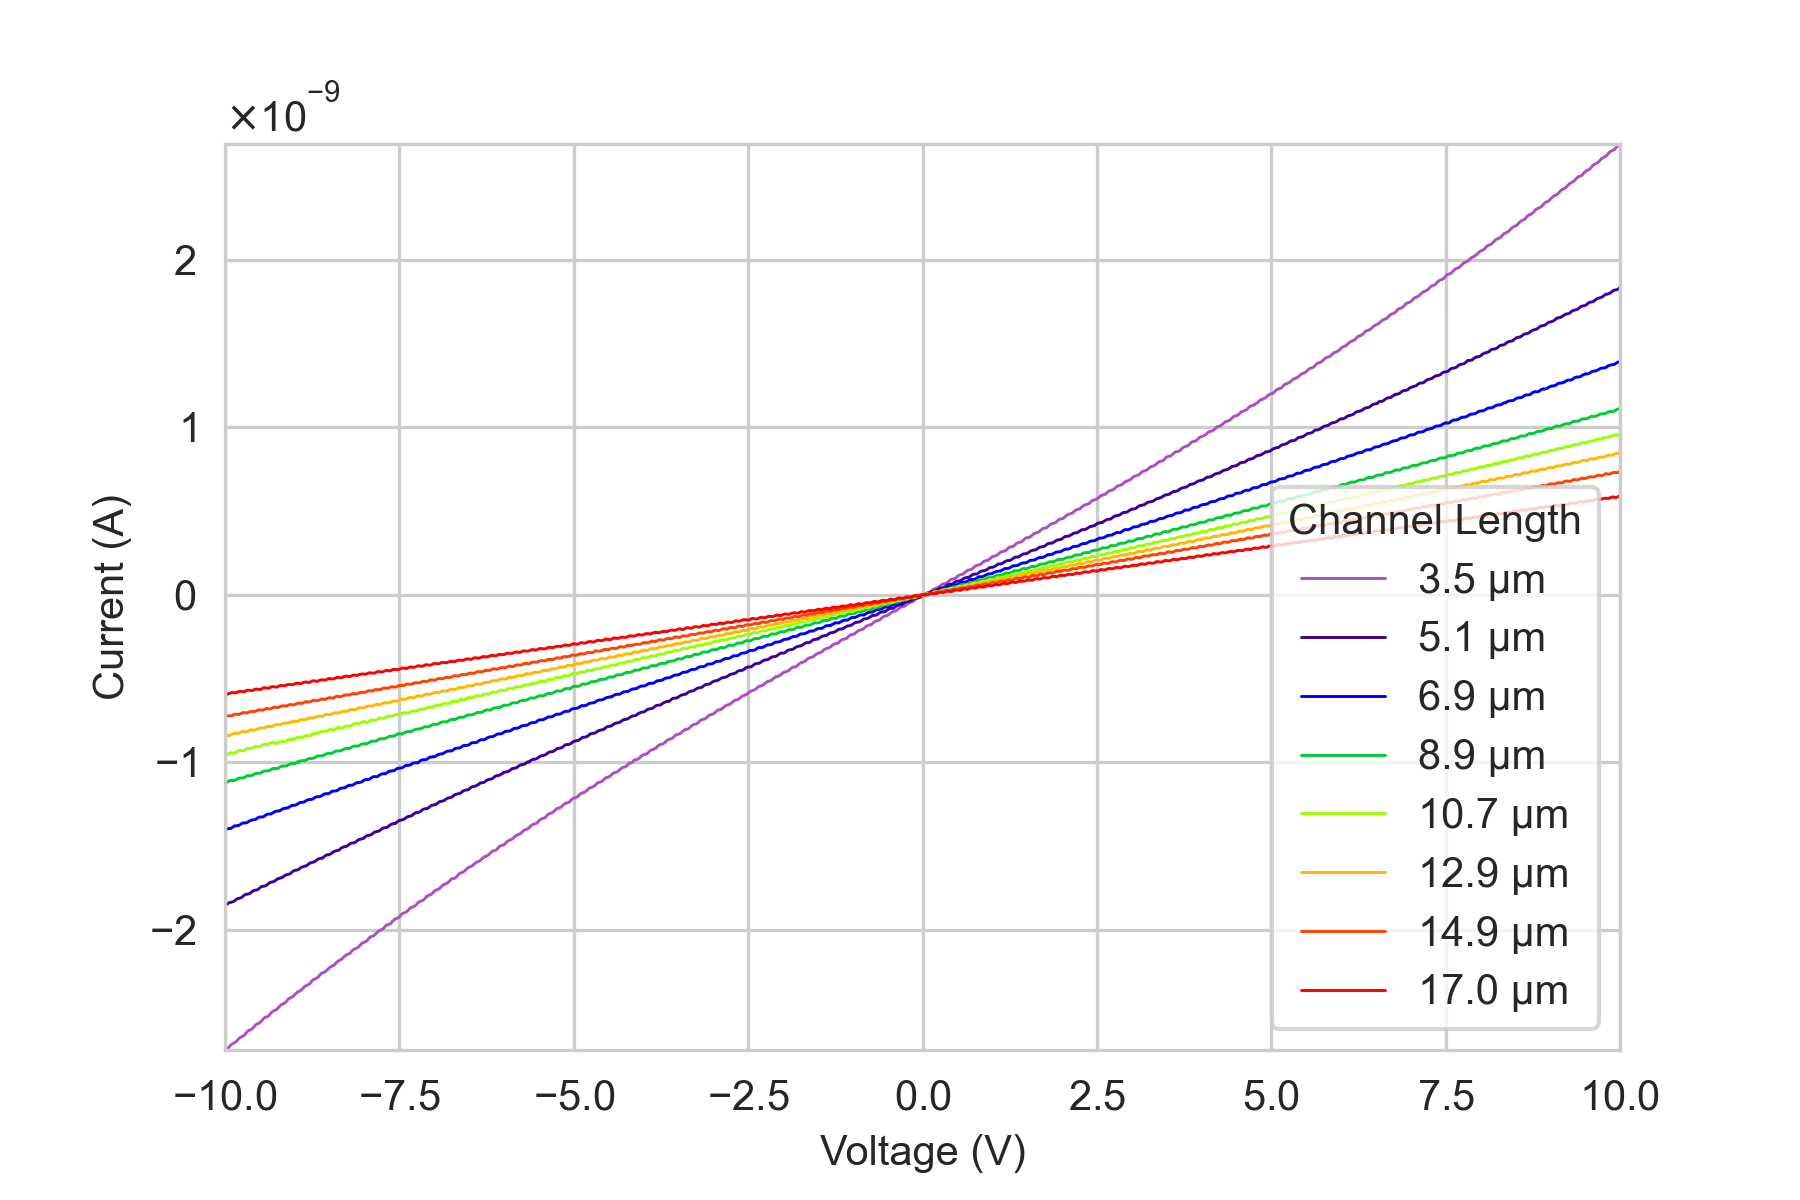
\includegraphics[width=0.97\textwidth]{Chapter6/Figs/Raster/Sample C 2019/IV/10V IV characteristics at 100 C.png}
    \caption{A linear plot of the measured current against applied voltage for all channel lengths at 100\si{\degreeCelsius} (sample C).}
    \label{appfig:C_current_voltage_100}
\end{figure}
\begin{figure}[h]
    \centering
    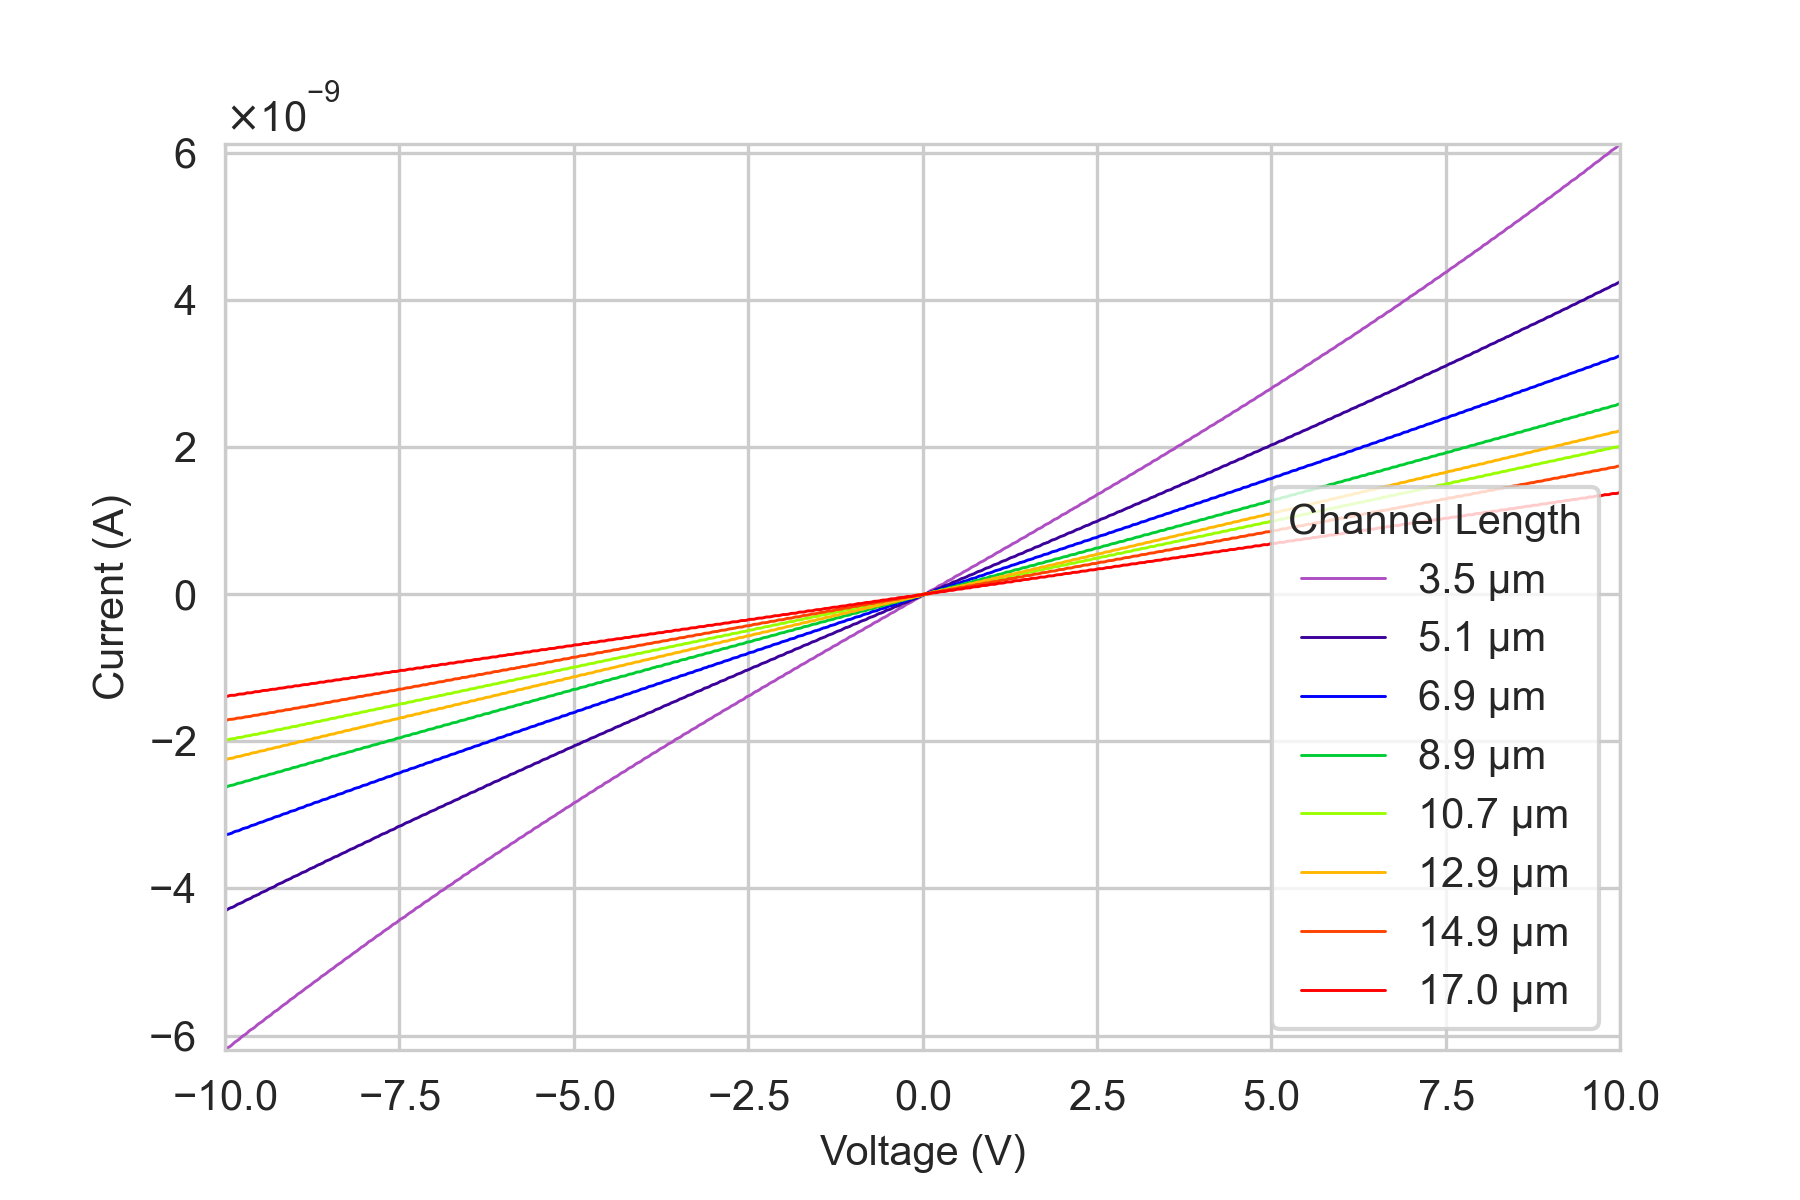
\includegraphics[width=0.97\textwidth]{Chapter6/Figs/Raster/Sample C 2019/IV/10V IV characteristics at 150 C.png}
    \caption{A linear plot of the measured current against applied voltage for all channel lengths at 150\si{\degreeCelsius} (sample C).}
    \label{appfig:C_current_voltage_150}
\end{figure}
\begin{figure}[h]
    \centering
    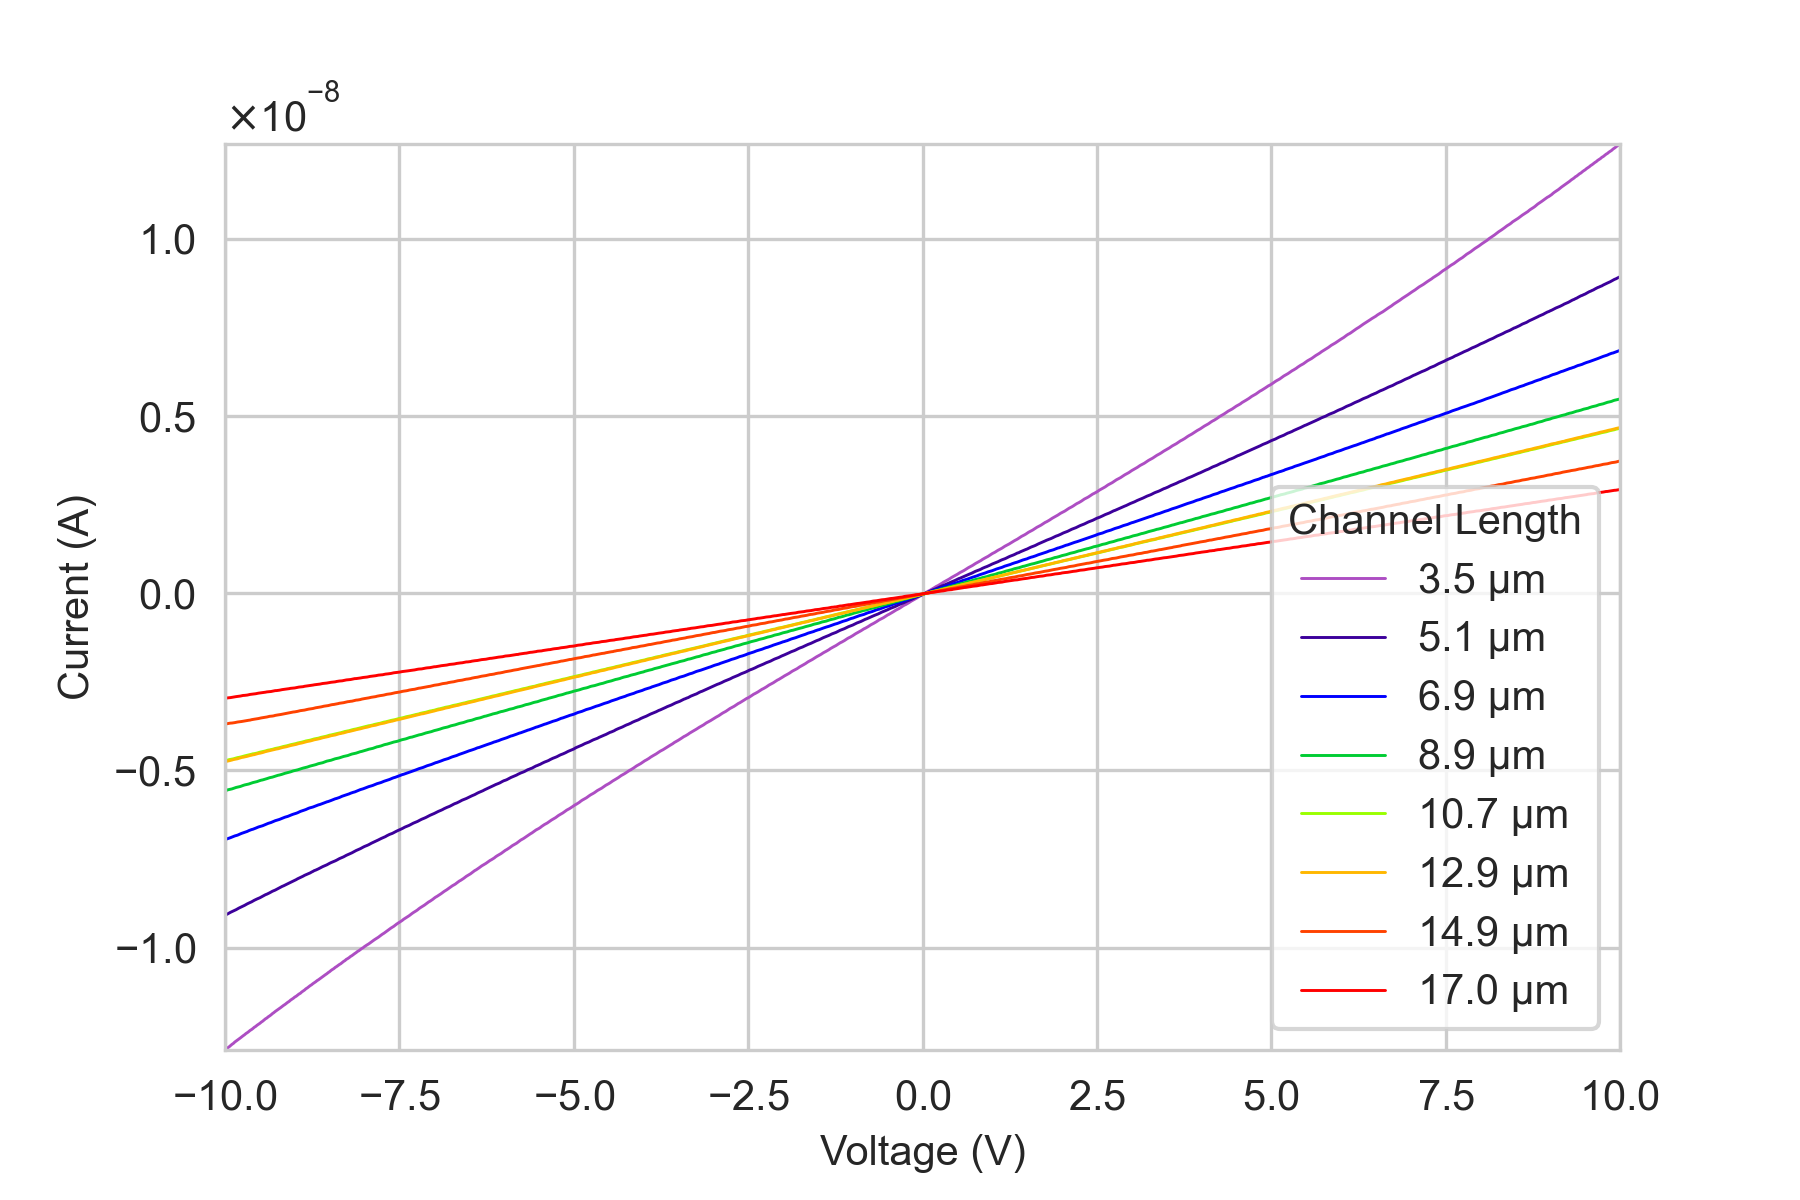
\includegraphics[width=0.97\textwidth]{Chapter6/Figs/Raster/Sample C 2019/IV/10V IV characteristics at 200 C.png}
    \caption{A linear plot of the measured current against applied voltage for all channel lengths at 200\si{\degreeCelsius} (sample C).}
    \label{appfig:C_current_voltage_200}
\end{figure}
\begin{figure}[h]
    \centering
    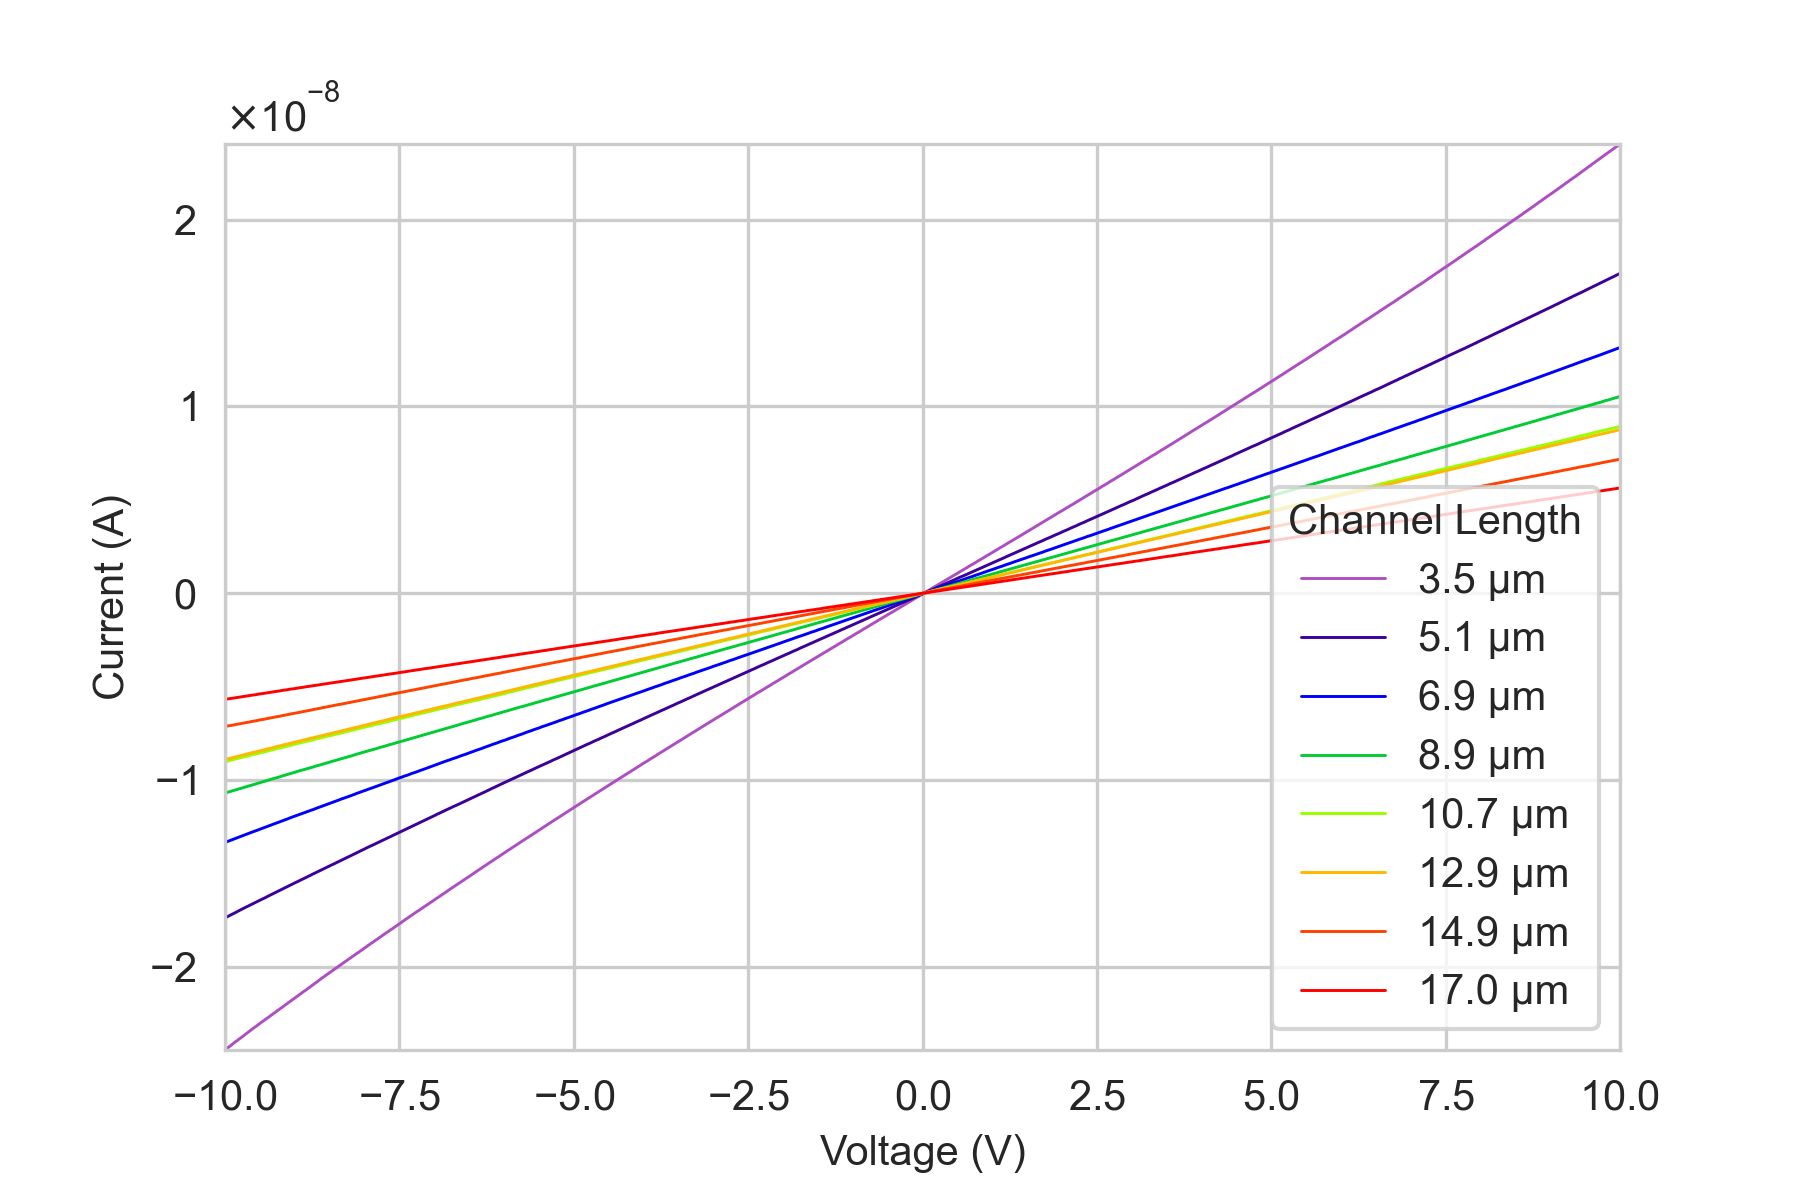
\includegraphics[width=0.97\textwidth]{Chapter6/Figs/Raster/Sample C 2019/IV/10V IV characteristics at 250 C.png}
    \caption{A linear plot of the measured current against applied voltage for all channel lengths at 250\si{\degreeCelsius} (sample C).}
    \label{appfig:C_current_voltage_250}
\end{figure}
\begin{figure}[h]
    \centering
    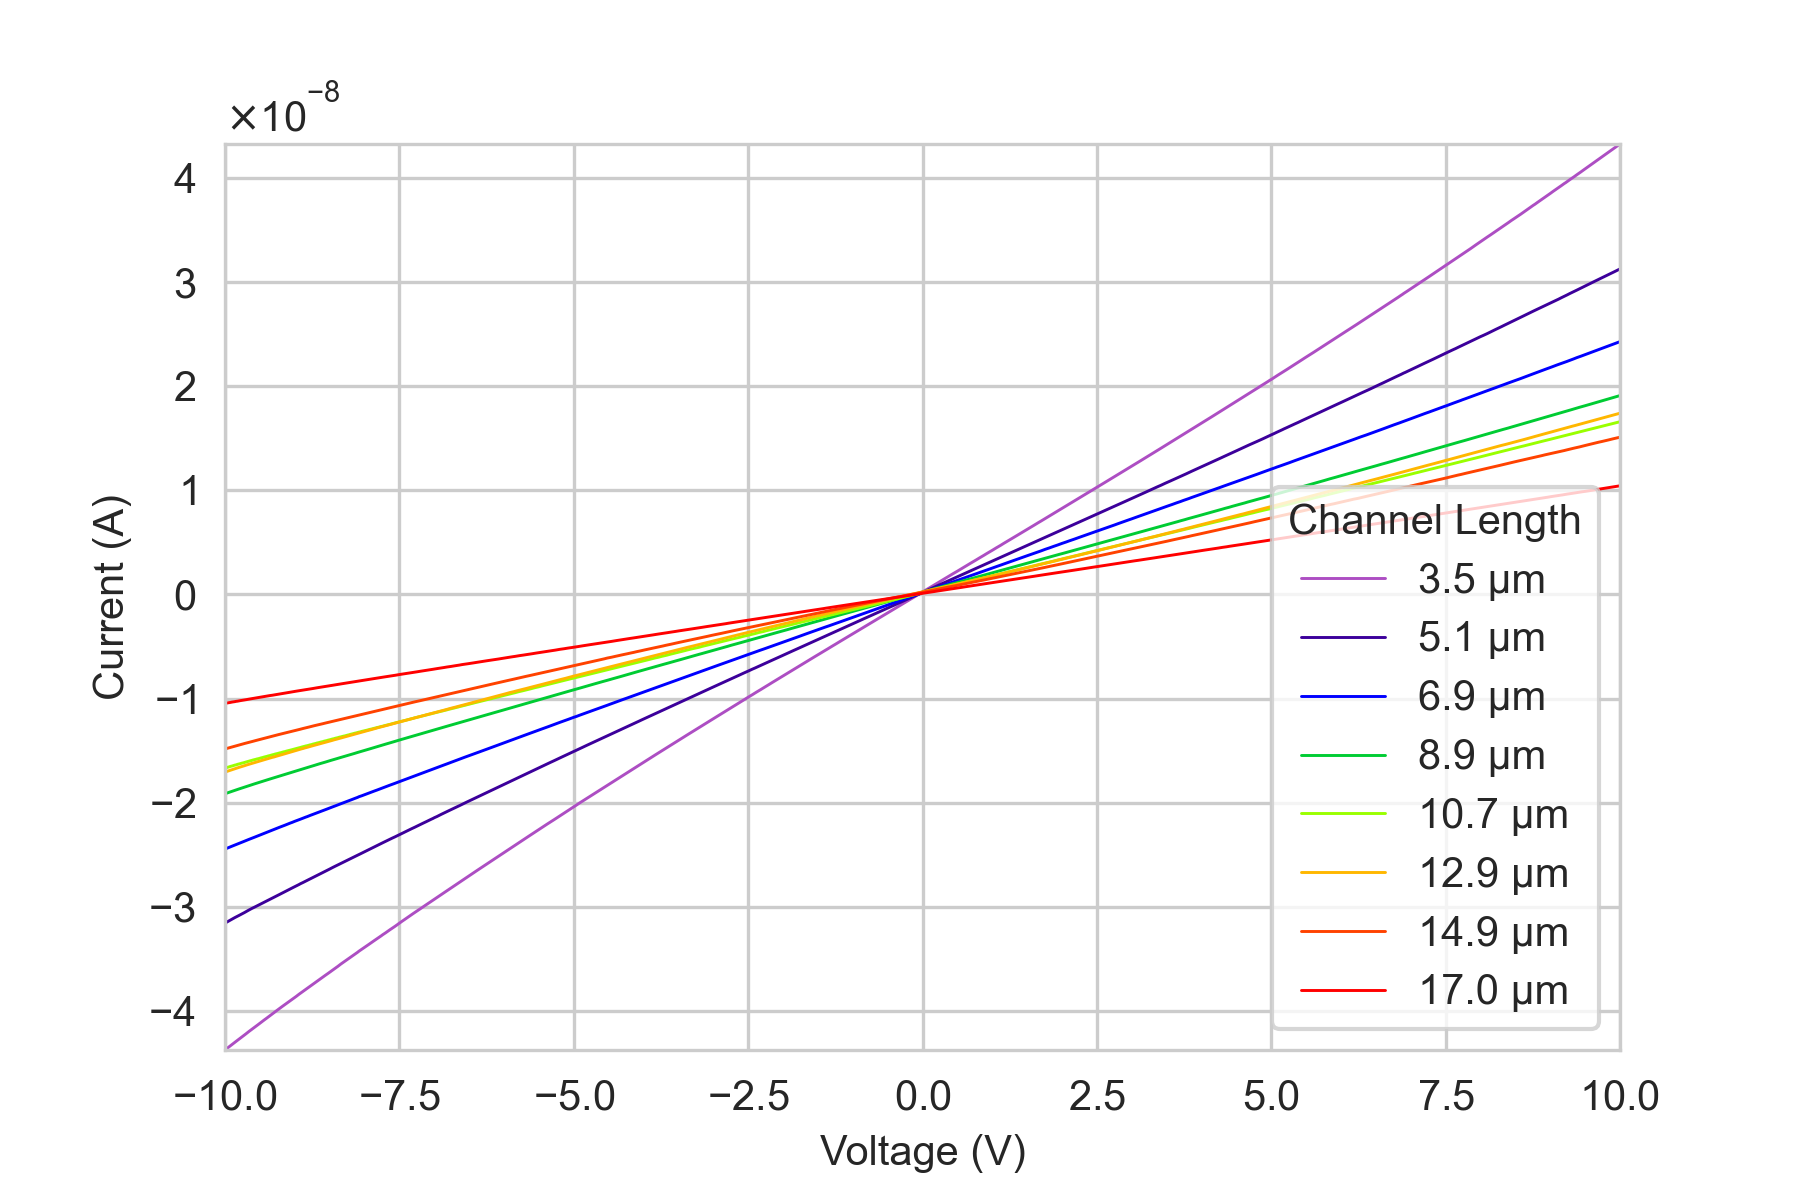
\includegraphics[width=0.97\textwidth]{Chapter6/Figs/Raster/Sample C 2019/IV/10V IV characteristics at 300 C.png}
    \caption{A linear plot of the measured current against applied voltage for all channel lengths at 300\si{\degreeCelsius} (sample C).}
    \label{appfig:C_current_voltage_300}
\end{figure}

\subsection{Sample D: 10 \si{\volt} range}

\label{app:I_V_sample_D_10V}
\begin{figure}[h]
    \centering
    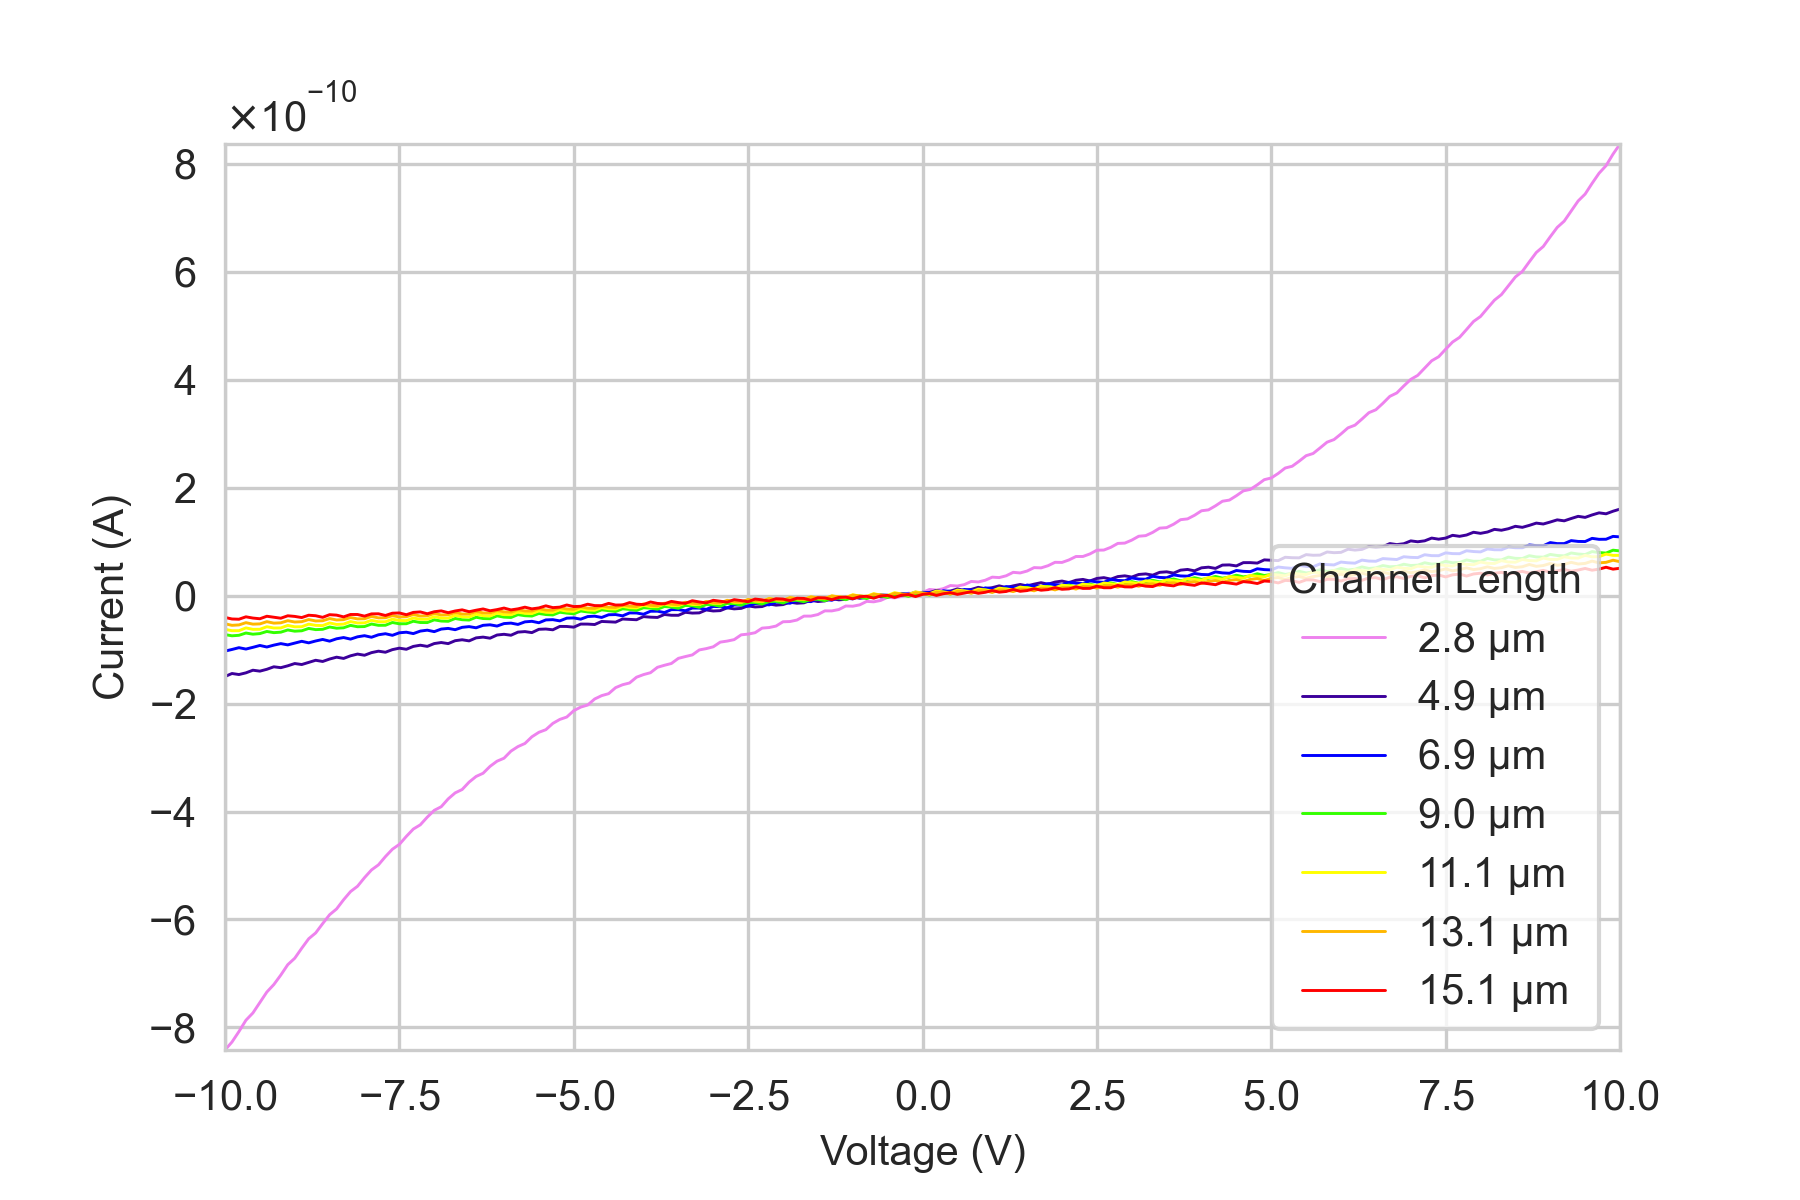
\includegraphics[width=0.97\textwidth]{Chapter6/Figs/Raster/Sample D 2019/IV/10V IV characteristics at 21 C.png}
    \caption{A linear plot of the measured current against applied voltage for all channel lengths at 21\si{\degreeCelsius} (sample D).}
    \label{appfig:D_current_voltage_21_10V}
\end{figure}
\begin{figure}[h]
    \centering
    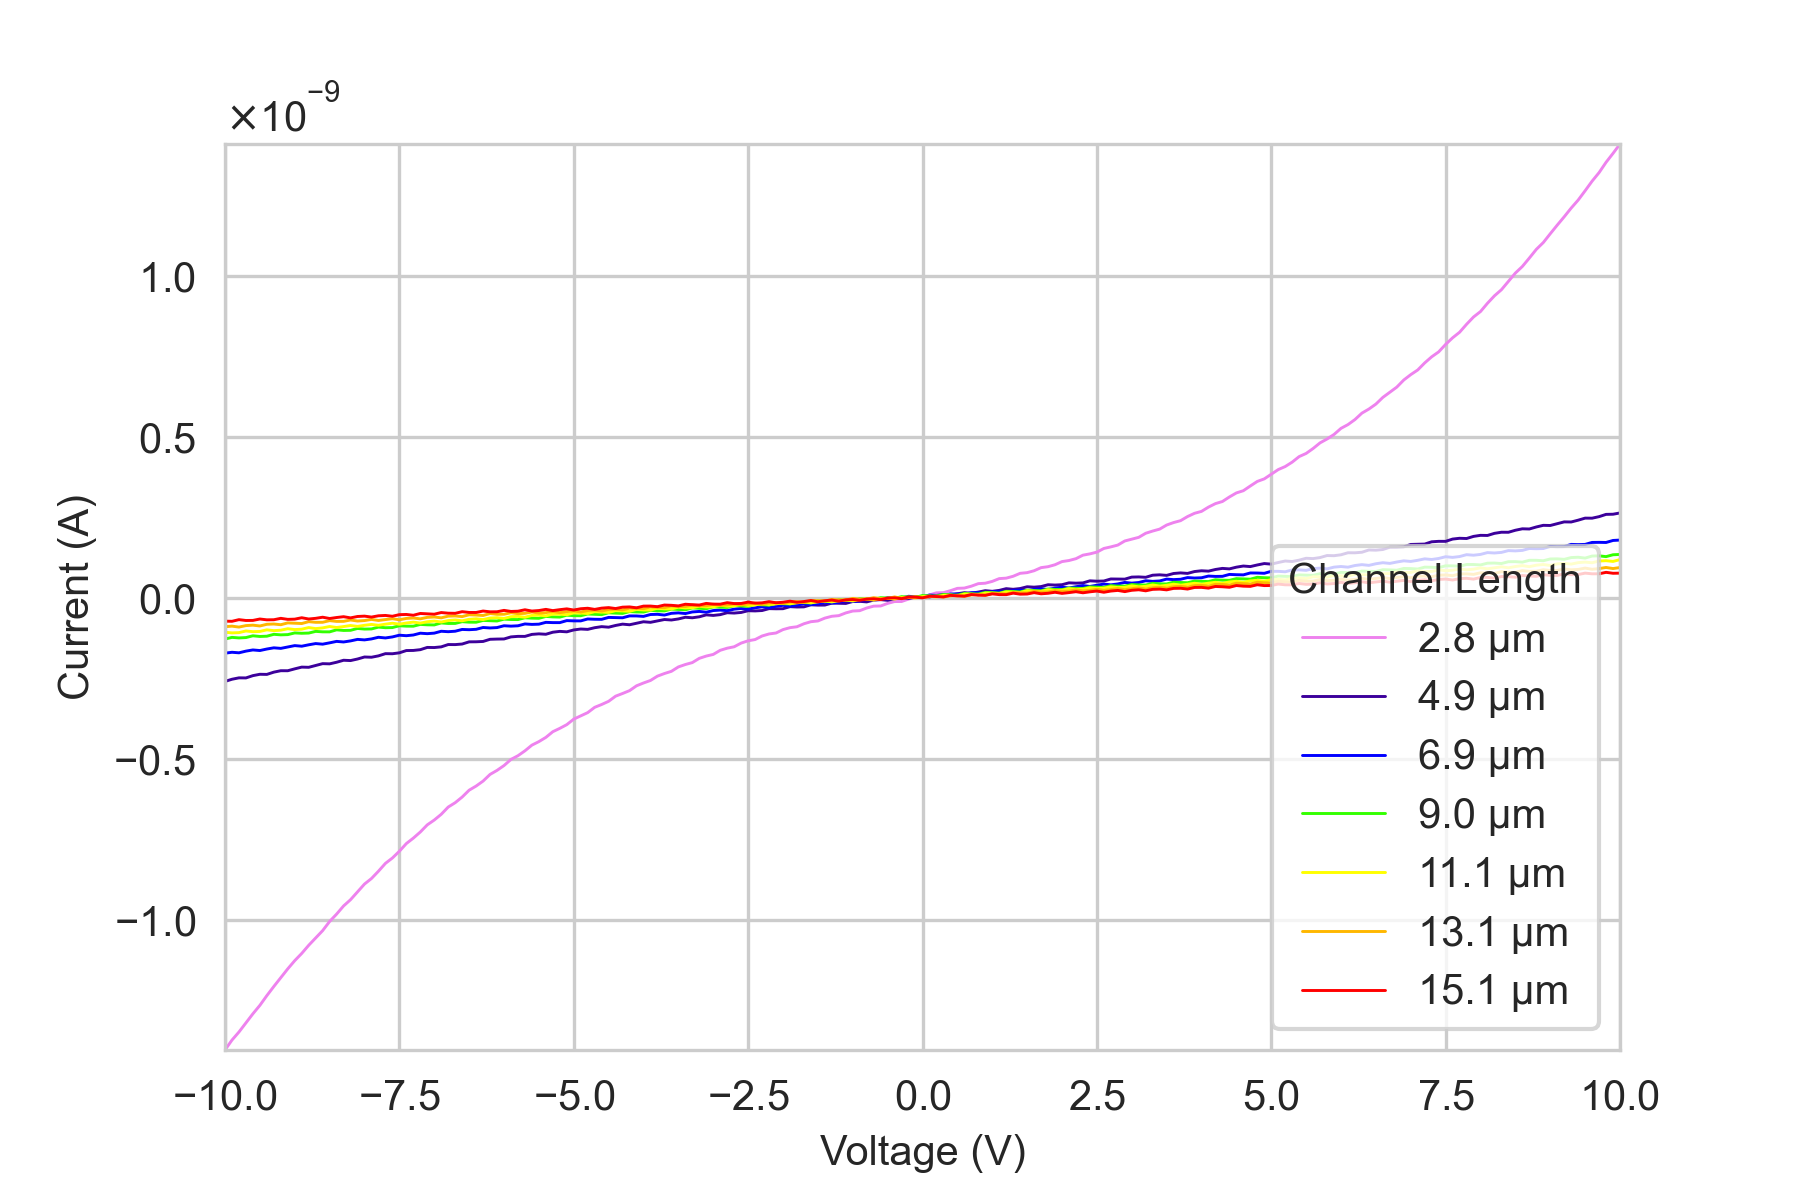
\includegraphics[width=0.97\textwidth]{Chapter6/Figs/Raster/Sample D 2019/IV/10V IV characteristics at 50 C.png}
    \caption{A linear plot of the measured current against applied voltage for all channel lengths at 50\si{\degreeCelsius} (sample D).}
    \label{appfig:D_current_voltage_50_10V}
\end{figure}
\begin{figure}[h]
    \centering
    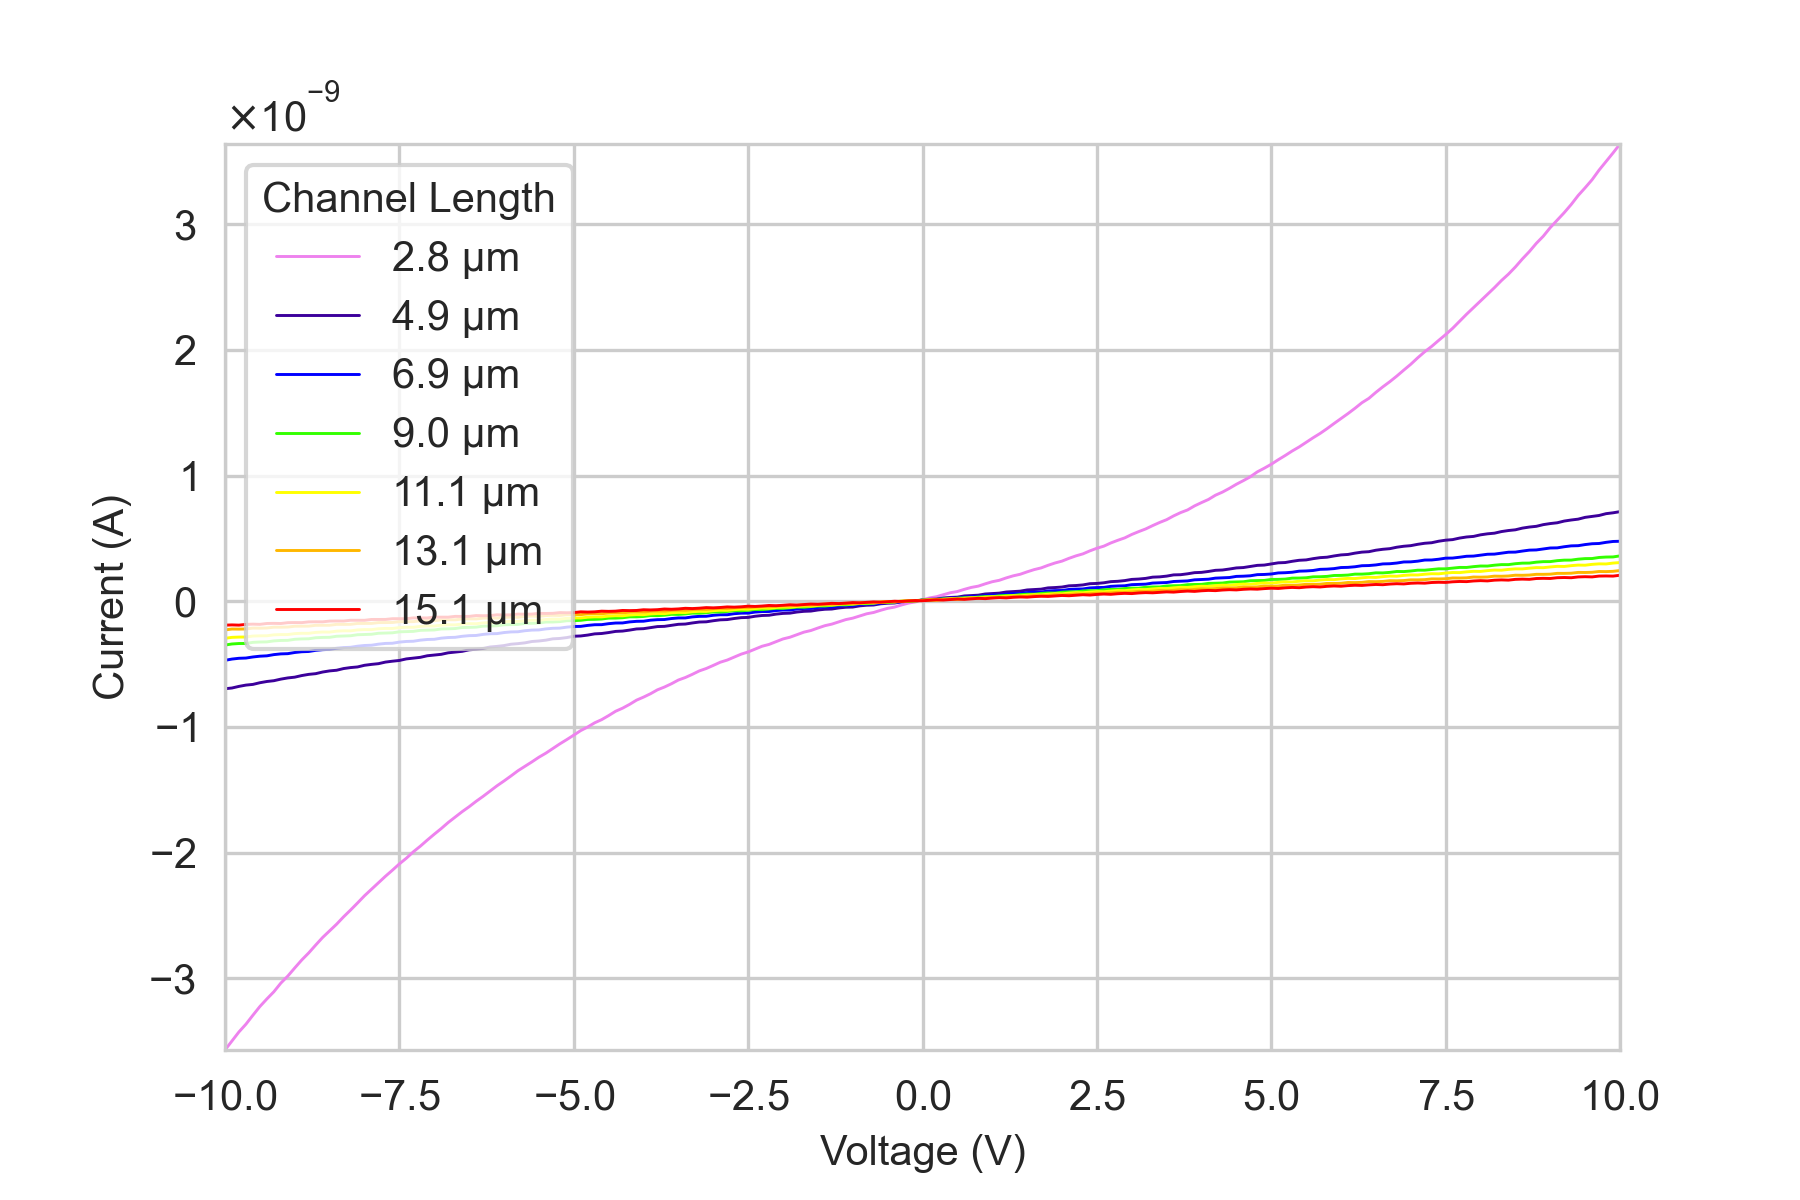
\includegraphics[width=0.97\textwidth]{Chapter6/Figs/Raster/Sample D 2019/IV/10V IV characteristics at 100 C.png}
    \caption{A linear plot of the measured current against applied voltage for all channel lengths at 100\si{\degreeCelsius} (sample D).}
    \label{appfig:D_current_voltage_100_10V}
\end{figure}
\begin{figure}[h]
    \centering
    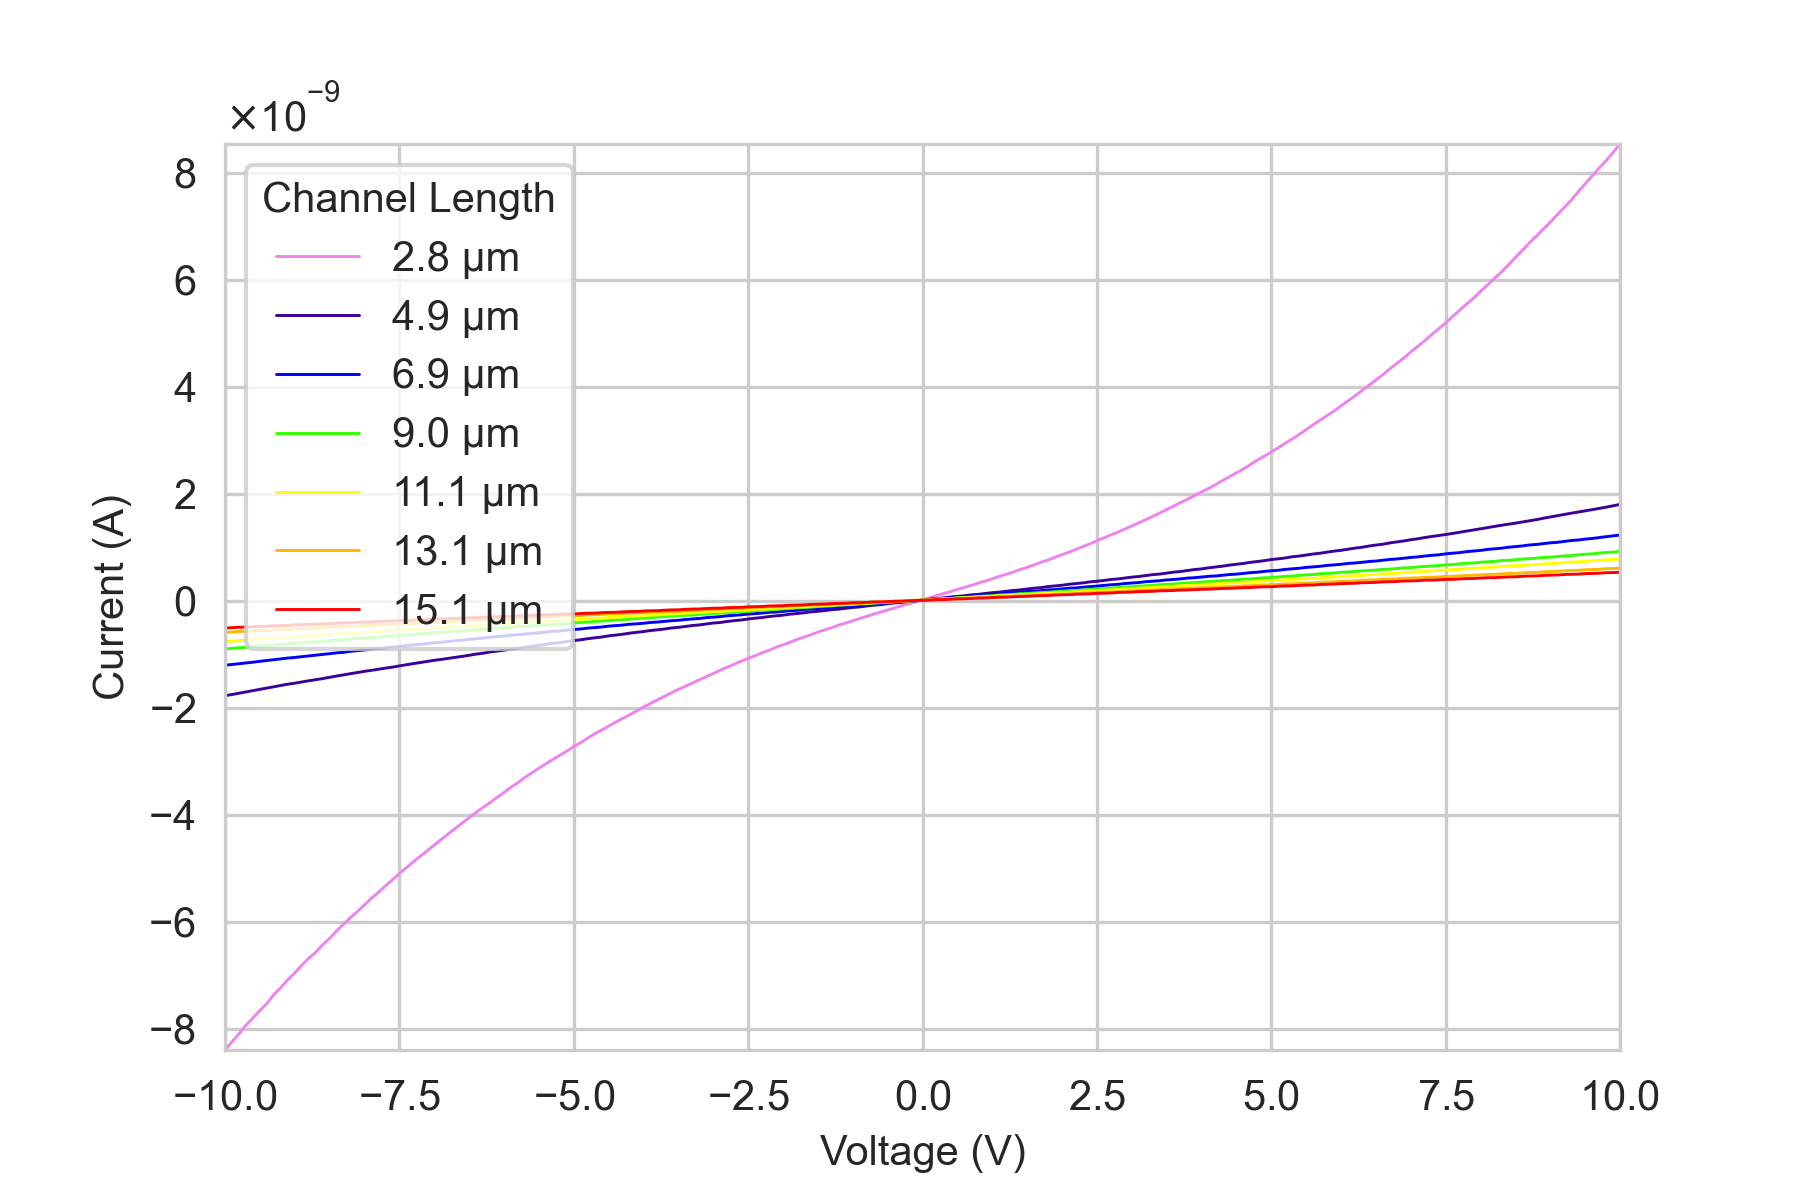
\includegraphics[width=0.97\textwidth]{Chapter6/Figs/Raster/Sample D 2019/IV/10V IV characteristics at 150 C.png}
    \caption{A linear plot of the measured current against applied voltage for all channel lengths at 150\si{\degreeCelsius} (sample D).}
    \label{appfig:D_current_voltage_150_10V}
\end{figure}
\begin{figure}[h]
    \centering
    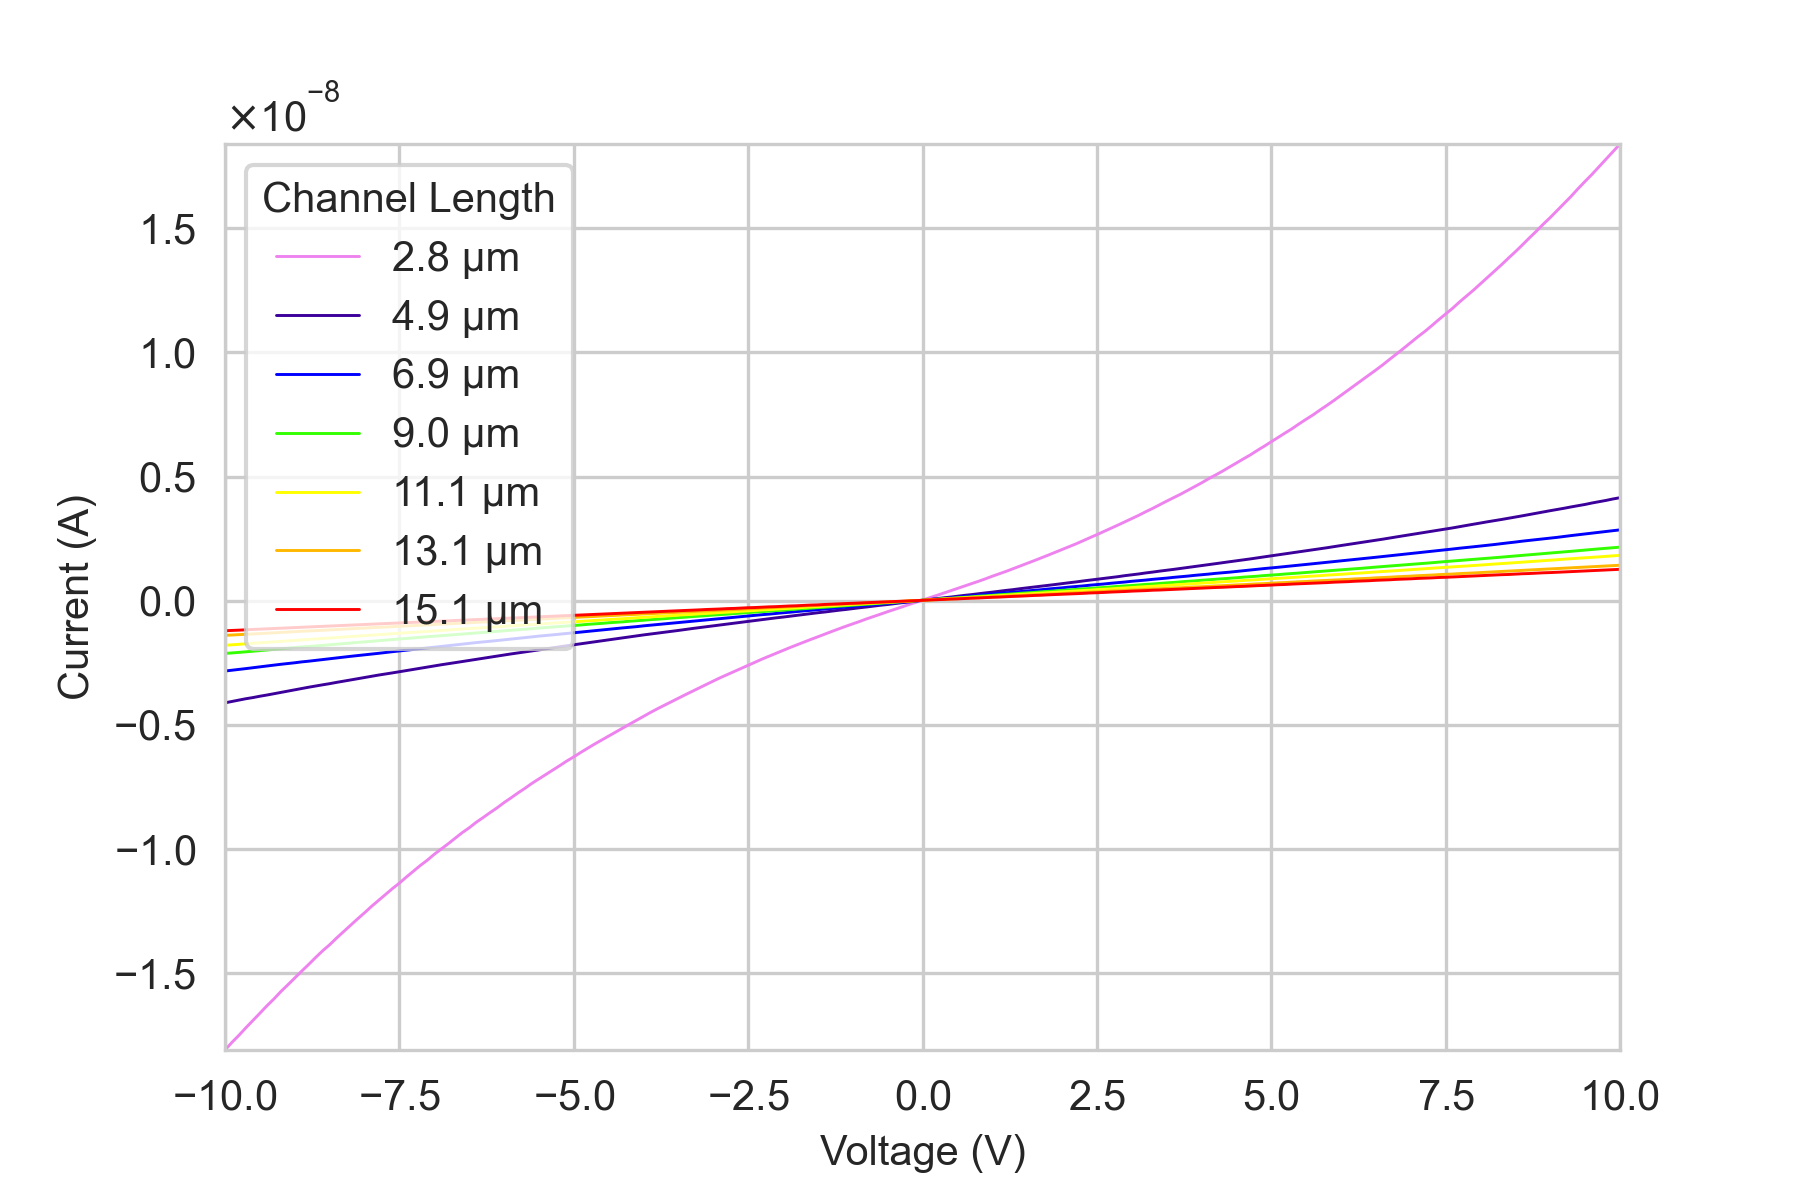
\includegraphics[width=0.97\textwidth]{Chapter6/Figs/Raster/Sample D 2019/IV/10V IV characteristics at 200 C.png}
    \caption{A linear plot of the measured current against applied voltage for all channel lengths at 200\si{\degreeCelsius} (sample D).}
    \label{appfig:D_current_voltage_200_10V}
\end{figure}
\begin{figure}[h]
    \centering
    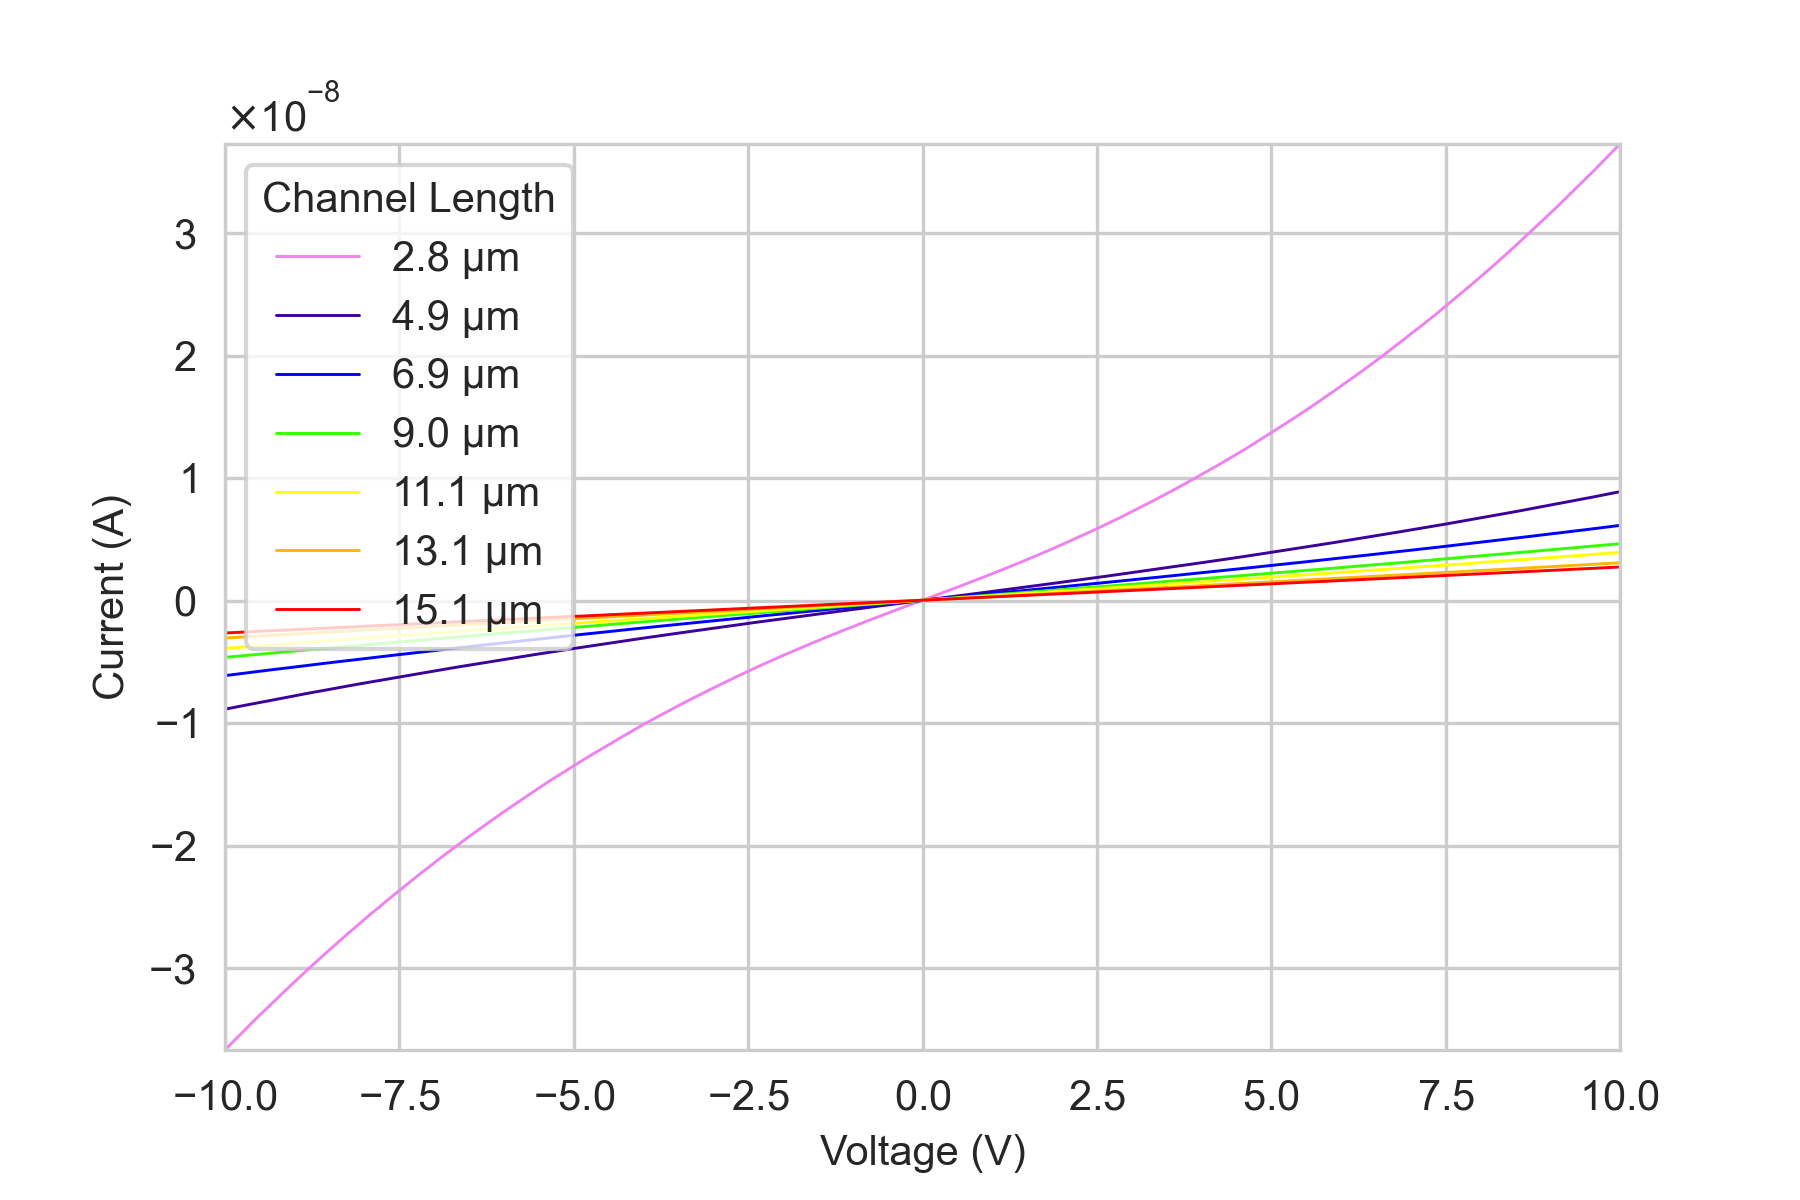
\includegraphics[width=0.97\textwidth]{Chapter6/Figs/Raster/Sample D 2019/IV/10V IV characteristics at 250 C.png}
    \caption{A linear plot of the measured current against applied voltage for all channel lengths at 250\si{\degreeCelsius} (sample D).}
    \label{appfig:D_current_voltage_250_10V}
\end{figure}
\begin{figure}[h]
    \centering
    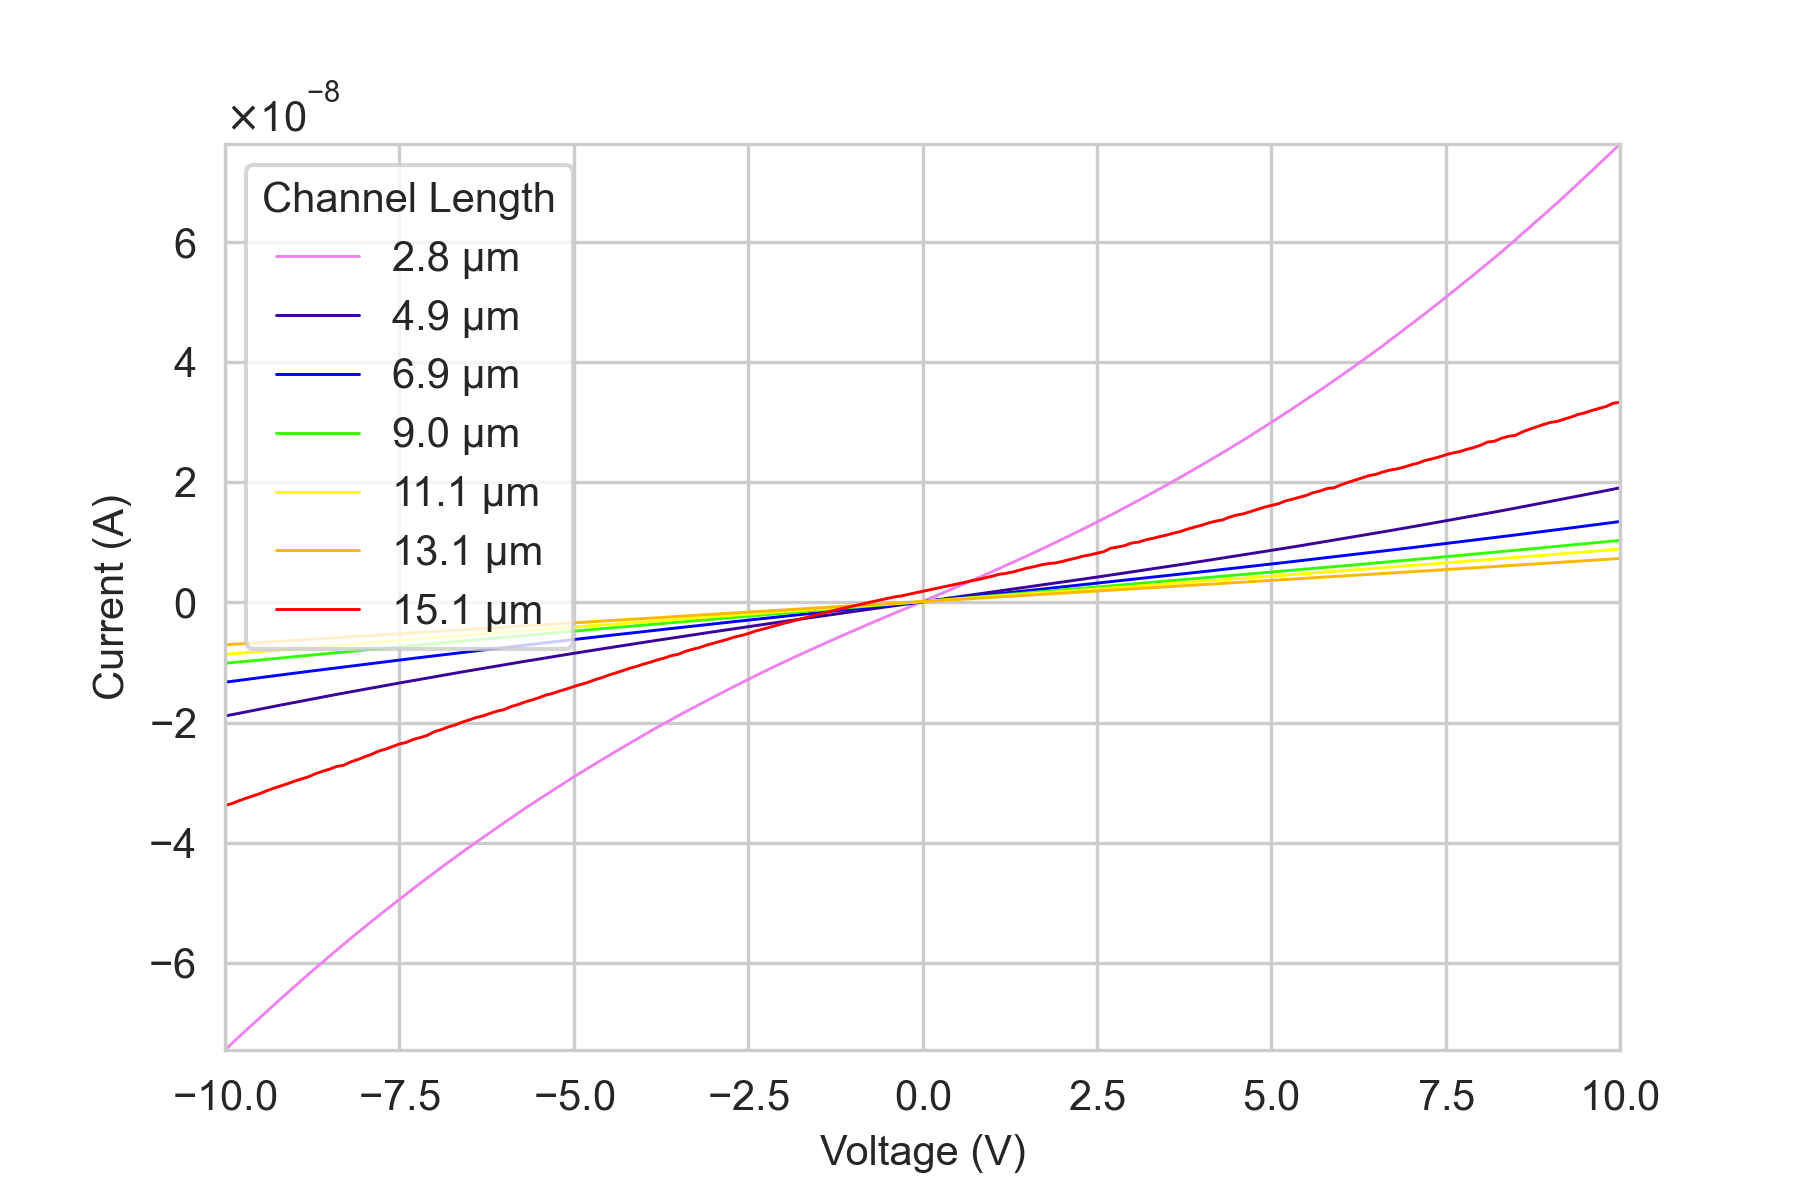
\includegraphics[width=0.97\textwidth]{Chapter6/Figs/Raster/Sample D 2019/IV/10V IV characteristics at 300 C.png}
    \caption{A linear plot of the measured current against applied voltage for all channel lengths at 300\si{\degreeCelsius} (sample D).}
    \label{appfig:D_current_voltage_300_10V}
\end{figure}